\chapter{Introduction}
\label{ch:intro}

\section{Churn in the telecommunication industry}

In recent years, the number of mobile phone users increased dramatically,
reaching more than 3 billion users worldwide. The number of mobile phone service
subscriptions is above the number of residents in several countries, including
Belgium \parencite{itu2018ict}. Telecommunication companies are evolving in a
saturated market, where customers are exposed to competitive offers from many
other companies. \textcite{hadden2007computer} show that attracting new
customers can be up to six times more expensive than retaining existing ones.
This led companies to switch from a selling-oriented to a customer-oriented
marketing approach. By building customer relationship based on trustworthiness
and commitment, a telecommunication company can reduce the incentives for their
client to churn, therefore increasing benefits through the subsequent customer
lifetime value.

One of the various marketing processes used to improve customer relationship is
to conduct retention campaigns. This traditionally consists in selecting clients
at random and offering them some a promotion or advantage. Typical promotions
include a reduced invoice, free calls, SMS or data volume. However, it is well
possible that the customers thus reached might never have planned to churn in
the first place. While this of course not a problem for the customer, it would
be far more beneficial for the telecommunication company to be able to focus the
retention campaigns on risky customers, in the hope of preventing attrition that
would otherwise occur if no action is taken. The problem of detecting churn can
be addressed with \emph{data mining}, by collecting data about customers and
using this information to infer typical patterns exhibited by risky clients.
This data-driven approach is nowadays taken by most major telecommunication
companies, and a part of the data mining literature is devoted to churn
detection. We will describe this approach further in the next section.



\section{Churn detection and prevention}

\begin{figure}[ht]
    \centering
    \includegraphics[width=0.8\linewidth]{figures/churn_diagram}
    \caption{The churn prevention process implemented at Orange.}
    \label{churn_diagram}
\end{figure}

The churn prevention process (depicted in figure \ref{churn_diagram}) starts by
collecting data about the customers and creating a \emph{historical database}.
This data summarizes the calls, messages, internet usage and other actions
performed by the customers. It also includes information about the subscription,
such as the type of tariff plan, its price, the subscription date, and so on.
Finally, personal data provided by the customer may as well be used, such as the
age or the place of residence. \emph{Data mining} is then used to provide a
quantitative understanding of the customers and their overall behavior. In
particular, the difference between churners and non-churners can be highlighted.
This is useful to decide which type of machine learning procedure should be used
for churn prediction, but can also bring valuable knowledge to marketing and
customer relationship teams. Once the data is sufficiently understood, a set of
relevant \emph{machine learning} models are built. These models learn from the
historical data the patterns typically exhibited by clients that will churn in
the near future. The types of patterns being learned, the techniques used to find
them, and the underlying assumptions are dependent on the model under
consideration. For example, a \emph{naive Bayes classifier} assumes that each
variable contributes to the probability of churn independently of the other
variables. In order to decide which model should be selected, the performances
of each model are compared by testing them on data left out of the training
phase. Feature selection is also performed, and consists in evaluating the
importance of each variable for predicting churn and training the model by
using only the most important ones. This reduces the computation time, and
generally improves the performances of the model since this reduces the noise
unimportant variables bring along. Once an efficient model has been selected,
the latest customer data is  submitted to the model, which outputs a probability
of churn for each customer. By ordering the customers by churn probability, a
list of the riskiest customers is established and sent to the campaigning team.
They split this set of clients into a \emph{target group} and a \emph{control
group}. Each customer of the target group is offered an incentive either by
phone call, email or message, while the control group is left untouched. This
allows, a few months later, to evaluate the impact of the retention campaign by
assessing the difference of churn rate in retrospective in the two groups.

\section{Causal inference}

Depending on the resources available and the techniques used, this data mining
pipeline can successfully predict potential churners, therefore allowing to
conduct targeted retention campaigns. But campaigners are then faced with
another challenge: what should they propose to the selected customers? Indeed,
the predictions given by data mining algorithms usually just consist in a
probability of churn. This prediction therefore does not indicate \emph{why} the
customer is about to stop her subscription. We need different analysis tools to
tackle this problem. This is the purpose of \emph{causal inference}, which is a
formal approach to find the causes of some event in a system. Causal inference
is usually conducted through \emph{controlled randomized experiments}, but the
scope of this master thesis did not allow such experiments. We therefore focus
on data-driven approaches, which are based on some properties of the statistical
distribution of causally linked variable.

To give an example of how causal inference can be conducted without experiment,
consider the simplistic world where two tariff plans are available, an expensive
one and a cheap one. The expensive plan makes customers consume more data per
month, and increases their probability to churn. We represent such causal
scenario with a \emph{directed acyclic graph} as in figure \ref{simple_causal}.
We plotted the data usage against the probability of churn for each tariff plan
in figure \ref{simple_causal_plot}. A positive correlation can be observed
between data usage and churn, but disappears when considering each tariff plan
separately. If a causal relationship also existed between data usage and churn
probability, the correlation would still be visible, even when conditioning on
the tariff plan. This idea of conditioning to discard putative causal links is
at the basis of most causal inference algorithms.

Such inference methods are based on a number of assumptions, such as the absence
of confounding factor. This assumption would be violated if, in our previous
example, the age of the customer influences both its choice of tariff plan and
its propensity  to churn. The causal inference algorithm would still conclude
that the expensive tariff plan causes clients to churn, while in reality they
churn solely because of their young age. This sort of erroneous conclusions can
lead to ineffective action in retention campaigns. Other inference methods imply
other assumptions, and care must be exercised when using them.

\begin{figure}
    \centering
    \begin{tikzpicture}
        \begin{scope}[every node/.style={ellipse,thick,draw}]
            \node (1) at (0, 0) {Tariff plan};
            \node[below left = of 1] (2) {Data usage};
            \node[below right = of 1] (3) {Churn};
        \end{scope}
        \begin{scope}[>={Stealth[black]},
            every edge/.style={draw=black,very thick}]
            \path [->] (1) edge node {} (3);
            \path [->] (1) edge node {} (2);
        \end{scope}
    \end{tikzpicture}
    \caption{Toy example of a causal diagram.}
    \label{simple_causal}
\end{figure}

\begin{figure}
    \centering
    % Created by tikzDevice version 0.12 on 2019-04-22 16:51:04
% !TEX encoding = UTF-8 Unicode
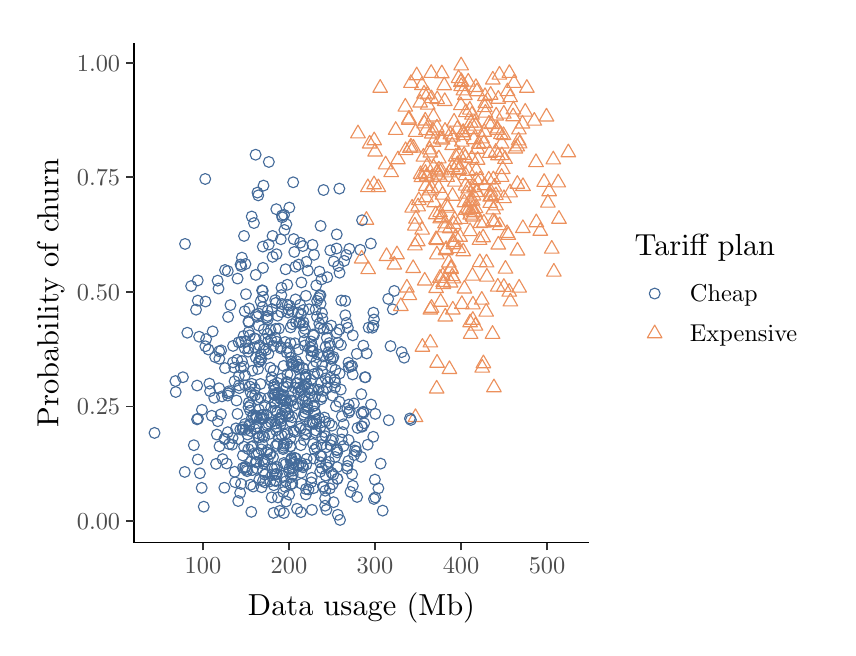
\begin{tikzpicture}[x=1pt,y=1pt]
\definecolor{fillColor}{RGB}{255,255,255}
\path[use as bounding box,fill=fillColor,fill opacity=0.00] (0,0) rectangle (289.08,216.81);
\begin{scope}
\path[clip] (  0.00,  0.00) rectangle (289.08,216.81);
\definecolor{drawColor}{RGB}{255,255,255}
\definecolor{fillColor}{RGB}{255,255,255}

\path[draw=drawColor,line width= 0.6pt,line join=round,line cap=round,fill=fillColor] (  0.00,  0.00) rectangle (289.08,216.81);
\end{scope}
\begin{scope}
\path[clip] ( 38.36, 30.72) rectangle (202.84,211.31);
\definecolor{fillColor}{RGB}{255,255,255}

\path[fill=fillColor] ( 38.36, 30.72) rectangle (202.84,211.31);
\definecolor{drawColor}{RGB}{236,144,92}

\path[draw=drawColor,line width= 0.4pt,line join=round,line cap=round] (147.98,193.93) --
	(150.62,189.35) --
	(145.34,189.35) --
	(147.98,193.93);

\path[draw=drawColor,line width= 0.4pt,line join=round,line cap=round] (174.34,194.68) --
	(176.98,190.11) --
	(171.69,190.11) --
	(174.34,194.68);
\definecolor{drawColor}{RGB}{68,107,154}

\path[draw=drawColor,line width= 0.4pt,line join=round,line cap=round] ( 69.18, 86.52) circle (  1.96);

\path[draw=drawColor,line width= 0.4pt,line join=round,line cap=round] ( 90.06, 55.58) circle (  1.96);

\path[draw=drawColor,line width= 0.4pt,line join=round,line cap=round] ( 99.51,109.18) circle (  1.96);

\path[draw=drawColor,line width= 0.4pt,line join=round,line cap=round] ( 78.65, 58.16) circle (  1.96);

\path[draw=drawColor,line width= 0.4pt,line join=round,line cap=round] ( 83.03,157.22) circle (  1.96);
\definecolor{drawColor}{RGB}{236,144,92}

\path[draw=drawColor,line width= 0.4pt,line join=round,line cap=round] (177.60,125.85) --
	(180.24,121.27) --
	(174.96,121.27) --
	(177.60,125.85);
\definecolor{drawColor}{RGB}{68,107,154}

\path[draw=drawColor,line width= 0.4pt,line join=round,line cap=round] ( 97.34, 42.96) circle (  1.96);

\path[draw=drawColor,line width= 0.4pt,line join=round,line cap=round] ( 92.57, 41.44) circle (  1.96);
\definecolor{drawColor}{RGB}{236,144,92}

\path[draw=drawColor,line width= 0.4pt,line join=round,line cap=round] (164.21,179.75) --
	(166.86,175.18) --
	(161.57,175.18) --
	(164.21,179.75);
\definecolor{drawColor}{RGB}{68,107,154}

\path[draw=drawColor,line width= 0.4pt,line join=round,line cap=round] ( 68.70, 74.60) circle (  1.96);

\path[draw=drawColor,line width= 0.4pt,line join=round,line cap=round] ( 93.89, 81.36) circle (  1.96);

\path[draw=drawColor,line width= 0.4pt,line join=round,line cap=round] ( 93.34, 52.90) circle (  1.96);

\path[draw=drawColor,line width= 0.4pt,line join=round,line cap=round] ( 94.98, 65.55) circle (  1.96);

\path[draw=drawColor,line width= 0.4pt,line join=round,line cap=round] ( 93.56, 99.48) circle (  1.96);

\path[draw=drawColor,line width= 0.4pt,line join=round,line cap=round] (108.64, 99.53) circle (  1.96);

\path[draw=drawColor,line width= 0.4pt,line join=round,line cap=round] ( 82.90,112.31) circle (  1.96);
\definecolor{drawColor}{RGB}{236,144,92}

\path[draw=drawColor,line width= 0.4pt,line join=round,line cap=round] (150.52,198.95) --
	(153.16,194.37) --
	(147.88,194.37) --
	(150.52,198.95);
\definecolor{drawColor}{RGB}{68,107,154}

\path[draw=drawColor,line width= 0.4pt,line join=round,line cap=round] (104.34, 75.20) circle (  1.96);

\path[draw=drawColor,line width= 0.4pt,line join=round,line cap=round] (100.13, 79.29) circle (  1.96);
\definecolor{drawColor}{RGB}{236,144,92}

\path[draw=drawColor,line width= 0.4pt,line join=round,line cap=round] (127.38,198.05) --
	(130.02,193.47) --
	(124.74,193.47) --
	(127.38,198.05);
\definecolor{drawColor}{RGB}{68,107,154}

\path[draw=drawColor,line width= 0.4pt,line join=round,line cap=round] ( 77.10, 51.93) circle (  1.96);
\definecolor{drawColor}{RGB}{236,144,92}

\path[draw=drawColor,line width= 0.4pt,line join=round,line cap=round] (166.98,174.53) --
	(169.63,169.95) --
	(164.34,169.95) --
	(166.98,174.53);
\definecolor{drawColor}{RGB}{68,107,154}

\path[draw=drawColor,line width= 0.4pt,line join=round,line cap=round] (103.42,105.60) circle (  1.96);

\path[draw=drawColor,line width= 0.4pt,line join=round,line cap=round] ( 76.50, 86.56) circle (  1.96);
\definecolor{drawColor}{RGB}{236,144,92}

\path[draw=drawColor,line width= 0.4pt,line join=round,line cap=round] (139.30,132.91) --
	(141.94,128.34) --
	(136.65,128.34) --
	(139.30,132.91);

\path[draw=drawColor,line width= 0.4pt,line join=round,line cap=round] (167.97,109.13) --
	(170.61,104.56) --
	(165.33,104.56) --
	(167.97,109.13);

\path[draw=drawColor,line width= 0.4pt,line join=round,line cap=round] (156.53,191.75) --
	(159.18,187.18) --
	(153.89,187.18) --
	(156.53,191.75);
\definecolor{drawColor}{RGB}{68,107,154}

\path[draw=drawColor,line width= 0.4pt,line join=round,line cap=round] ( 80.37, 78.42) circle (  1.96);

\path[draw=drawColor,line width= 0.4pt,line join=round,line cap=round] (106.19, 61.88) circle (  1.96);
\definecolor{drawColor}{RGB}{236,144,92}

\path[draw=drawColor,line width= 0.4pt,line join=round,line cap=round] (132.98,182.83) --
	(135.62,178.25) --
	(130.33,178.25) --
	(132.98,182.83);
\definecolor{drawColor}{RGB}{68,107,154}

\path[draw=drawColor,line width= 0.4pt,line join=round,line cap=round] ( 86.79, 64.24) circle (  1.96);
\definecolor{drawColor}{RGB}{236,144,92}

\path[draw=drawColor,line width= 0.4pt,line join=round,line cap=round] (133.80,172.21) --
	(136.44,167.64) --
	(131.16,167.64) --
	(133.80,172.21);
\definecolor{drawColor}{RGB}{68,107,154}

\path[draw=drawColor,line width= 0.4pt,line join=round,line cap=round] (112.18,130.69) circle (  1.96);

\path[draw=drawColor,line width= 0.4pt,line join=round,line cap=round] (107.86, 58.88) circle (  1.96);
\definecolor{drawColor}{RGB}{236,144,92}

\path[draw=drawColor,line width= 0.4pt,line join=round,line cap=round] (156.71,200.47) --
	(159.35,195.90) --
	(154.07,195.90) --
	(156.71,200.47);
\definecolor{drawColor}{RGB}{68,107,154}

\path[draw=drawColor,line width= 0.4pt,line join=round,line cap=round] ( 80.98, 88.11) circle (  1.96);
\definecolor{drawColor}{RGB}{236,144,92}

\path[draw=drawColor,line width= 0.4pt,line join=round,line cap=round] (174.06,203.41) --
	(176.71,198.83) --
	(171.42,198.83) --
	(174.06,203.41);
\definecolor{drawColor}{RGB}{68,107,154}

\path[draw=drawColor,line width= 0.4pt,line join=round,line cap=round] ( 80.81, 41.85) circle (  1.96);

\path[draw=drawColor,line width= 0.4pt,line join=round,line cap=round] (104.54,112.35) circle (  1.96);
\definecolor{drawColor}{RGB}{236,144,92}

\path[draw=drawColor,line width= 0.4pt,line join=round,line cap=round] (125.22,179.08) --
	(127.86,174.51) --
	(122.58,174.51) --
	(125.22,179.08);

\path[draw=drawColor,line width= 0.4pt,line join=round,line cap=round] (140.58,202.54) --
	(143.22,197.97) --
	(137.94,197.97) --
	(140.58,202.54);

\path[draw=drawColor,line width= 0.4pt,line join=round,line cap=round] (152.93,132.96) --
	(155.57,128.38) --
	(150.28,128.38) --
	(152.93,132.96);
\definecolor{drawColor}{RGB}{68,107,154}

\path[draw=drawColor,line width= 0.4pt,line join=round,line cap=round] (119.04, 47.24) circle (  1.96);
\definecolor{drawColor}{RGB}{236,144,92}

\path[draw=drawColor,line width= 0.4pt,line join=round,line cap=round] (173.24,145.55) --
	(175.88,140.98) --
	(170.59,140.98) --
	(173.24,145.55);
\definecolor{drawColor}{RGB}{68,107,154}

\path[draw=drawColor,line width= 0.4pt,line join=round,line cap=round] ( 76.83, 71.63) circle (  1.96);

\path[draw=drawColor,line width= 0.4pt,line join=round,line cap=round] (128.28, 42.30) circle (  1.96);

\path[draw=drawColor,line width= 0.4pt,line join=round,line cap=round] (113.20,102.14) circle (  1.96);

\path[draw=drawColor,line width= 0.4pt,line join=round,line cap=round] ( 64.25,117.85) circle (  1.96);

\path[draw=drawColor,line width= 0.4pt,line join=round,line cap=round] (121.39, 77.66) circle (  1.96);

\path[draw=drawColor,line width= 0.4pt,line join=round,line cap=round] ( 98.68, 71.96) circle (  1.96);

\path[draw=drawColor,line width= 0.4pt,line join=round,line cap=round] (103.09, 99.82) circle (  1.96);

\path[draw=drawColor,line width= 0.4pt,line join=round,line cap=round] ( 82.38, 59.81) circle (  1.96);

\path[draw=drawColor,line width= 0.4pt,line join=round,line cap=round] (100.64, 69.92) circle (  1.96);
\definecolor{drawColor}{RGB}{236,144,92}

\path[draw=drawColor,line width= 0.4pt,line join=round,line cap=round] (153.88,142.32) --
	(156.52,137.74) --
	(151.24,137.74) --
	(153.88,142.32);
\definecolor{drawColor}{RGB}{68,107,154}

\path[draw=drawColor,line width= 0.4pt,line join=round,line cap=round] (100.26, 77.77) circle (  1.96);

\path[draw=drawColor,line width= 0.4pt,line join=round,line cap=round] ( 84.19,117.89) circle (  1.96);

\path[draw=drawColor,line width= 0.4pt,line join=round,line cap=round] ( 72.43,112.28) circle (  1.96);

\path[draw=drawColor,line width= 0.4pt,line join=round,line cap=round] (110.19, 83.85) circle (  1.96);

\path[draw=drawColor,line width= 0.4pt,line join=round,line cap=round] ( 94.92, 68.31) circle (  1.96);
\definecolor{drawColor}{RGB}{236,144,92}

\path[draw=drawColor,line width= 0.4pt,line join=round,line cap=round] (186.63,164.04) --
	(189.27,159.47) --
	(183.99,159.47) --
	(186.63,164.04);
\definecolor{drawColor}{RGB}{68,107,154}

\path[draw=drawColor,line width= 0.4pt,line join=round,line cap=round] ( 89.37, 86.03) circle (  1.96);

\path[draw=drawColor,line width= 0.4pt,line join=round,line cap=round] ( 82.71, 59.87) circle (  1.96);

\path[draw=drawColor,line width= 0.4pt,line join=round,line cap=round] (105.97, 82.53) circle (  1.96);
\definecolor{drawColor}{RGB}{236,144,92}

\path[draw=drawColor,line width= 0.4pt,line join=round,line cap=round] (138.93,154.75) --
	(141.57,150.18) --
	(136.28,150.18) --
	(138.93,154.75);

\path[draw=drawColor,line width= 0.4pt,line join=round,line cap=round] (173.38,196.81) --
	(176.02,192.23) --
	(170.74,192.23) --
	(173.38,196.81);
\definecolor{drawColor}{RGB}{68,107,154}

\path[draw=drawColor,line width= 0.4pt,line join=round,line cap=round] ( 86.74,112.68) circle (  1.96);

\path[draw=drawColor,line width= 0.4pt,line join=round,line cap=round] ( 86.67,114.46) circle (  1.96);

\path[draw=drawColor,line width= 0.4pt,line join=round,line cap=round] ( 68.06, 59.17) circle (  1.96);

\path[draw=drawColor,line width= 0.4pt,line join=round,line cap=round] (104.01,115.00) circle (  1.96);

\path[draw=drawColor,line width= 0.4pt,line join=round,line cap=round] ( 85.02, 60.71) circle (  1.96);

\path[draw=drawColor,line width= 0.4pt,line join=round,line cap=round] ( 83.43, 63.14) circle (  1.96);

\path[draw=drawColor,line width= 0.4pt,line join=round,line cap=round] (115.70,108.36) circle (  1.96);

\path[draw=drawColor,line width= 0.4pt,line join=round,line cap=round] (108.25,126.65) circle (  1.96);

\path[draw=drawColor,line width= 0.4pt,line join=round,line cap=round] ( 79.84,110.33) circle (  1.96);

\path[draw=drawColor,line width= 0.4pt,line join=round,line cap=round] (103.26, 50.40) circle (  1.96);
\definecolor{drawColor}{RGB}{236,144,92}

\path[draw=drawColor,line width= 0.4pt,line join=round,line cap=round] (147.88,137.85) --
	(150.52,133.28) --
	(145.23,133.28) --
	(147.88,137.85);
\definecolor{drawColor}{RGB}{68,107,154}

\path[draw=drawColor,line width= 0.4pt,line join=round,line cap=round] ( 84.71, 75.31) circle (  1.96);
\definecolor{drawColor}{RGB}{236,144,92}

\path[draw=drawColor,line width= 0.4pt,line join=round,line cap=round] (189.37,139.91) --
	(192.01,135.33) --
	(186.73,135.33) --
	(189.37,139.91);
\definecolor{drawColor}{RGB}{68,107,154}

\path[draw=drawColor,line width= 0.4pt,line join=round,line cap=round] ( 84.13, 88.06) circle (  1.96);

\path[draw=drawColor,line width= 0.4pt,line join=round,line cap=round] ( 66.52, 76.57) circle (  1.96);

\path[draw=drawColor,line width= 0.4pt,line join=round,line cap=round] (101.24,129.04) circle (  1.96);
\definecolor{drawColor}{RGB}{236,144,92}

\path[draw=drawColor,line width= 0.4pt,line join=round,line cap=round] (158.23,162.70) --
	(160.87,158.12) --
	(155.59,158.12) --
	(158.23,162.70);

\path[draw=drawColor,line width= 0.4pt,line join=round,line cap=round] (162.98,177.81) --
	(165.63,173.23) --
	(160.34,173.23) --
	(162.98,177.81);
\definecolor{drawColor}{RGB}{68,107,154}

\path[draw=drawColor,line width= 0.4pt,line join=round,line cap=round] ( 99.17, 86.25) circle (  1.96);

\path[draw=drawColor,line width= 0.4pt,line join=round,line cap=round] (125.46, 53.50) circle (  1.96);

\path[draw=drawColor,line width= 0.4pt,line join=round,line cap=round] (104.73, 98.81) circle (  1.96);

\path[draw=drawColor,line width= 0.4pt,line join=round,line cap=round] ( 94.89, 91.36) circle (  1.96);

\path[draw=drawColor,line width= 0.4pt,line join=round,line cap=round] ( 98.06,110.19) circle (  1.96);
\definecolor{drawColor}{RGB}{236,144,92}

\path[draw=drawColor,line width= 0.4pt,line join=round,line cap=round] (172.49,172.35) --
	(175.14,167.77) --
	(169.85,167.77) --
	(172.49,172.35);

\path[draw=drawColor,line width= 0.4pt,line join=round,line cap=round] (166.70,185.13) --
	(169.34,180.55) --
	(164.06,180.55) --
	(166.70,185.13);
\definecolor{drawColor}{RGB}{68,107,154}

\path[draw=drawColor,line width= 0.4pt,line join=round,line cap=round] (110.31, 68.12) circle (  1.96);

\path[draw=drawColor,line width= 0.4pt,line join=round,line cap=round] ( 64.16,162.14) circle (  1.96);

\path[draw=drawColor,line width= 0.4pt,line join=round,line cap=round] ( 87.98, 79.57) circle (  1.96);

\path[draw=drawColor,line width= 0.4pt,line join=round,line cap=round] (110.13, 97.27) circle (  1.96);
\definecolor{drawColor}{RGB}{236,144,92}

\path[draw=drawColor,line width= 0.4pt,line join=round,line cap=round] (137.69,186.50) --
	(140.34,181.92) --
	(135.05,181.92) --
	(137.69,186.50);
\definecolor{drawColor}{RGB}{68,107,154}

\path[draw=drawColor,line width= 0.4pt,line join=round,line cap=round] ( 59.07,123.43) circle (  1.96);
\definecolor{drawColor}{RGB}{236,144,92}

\path[draw=drawColor,line width= 0.4pt,line join=round,line cap=round] (148.03,167.80) --
	(150.68,163.22) --
	(145.39,163.22) --
	(148.03,167.80);

\path[draw=drawColor,line width= 0.4pt,line join=round,line cap=round] (146.01,181.53) --
	(148.66,176.95) --
	(143.37,176.95) --
	(146.01,181.53);
\definecolor{drawColor}{RGB}{68,107,154}

\path[draw=drawColor,line width= 0.4pt,line join=round,line cap=round] (109.59, 67.70) circle (  1.96);
\definecolor{drawColor}{RGB}{236,144,92}

\path[draw=drawColor,line width= 0.4pt,line join=round,line cap=round] (133.45,137.89) --
	(136.09,133.32) --
	(130.80,133.32) --
	(133.45,137.89);
\definecolor{drawColor}{RGB}{68,107,154}

\path[draw=drawColor,line width= 0.4pt,line join=round,line cap=round] (107.48, 44.07) circle (  1.96);

\path[draw=drawColor,line width= 0.4pt,line join=round,line cap=round] (115.91, 95.76) circle (  1.96);

\path[draw=drawColor,line width= 0.4pt,line join=round,line cap=round] (102.57, 85.79) circle (  1.96);
\definecolor{drawColor}{RGB}{236,144,92}

\path[draw=drawColor,line width= 0.4pt,line join=round,line cap=round] (187.98,156.54) --
	(190.62,151.97) --
	(185.33,151.97) --
	(187.98,156.54);
\definecolor{drawColor}{RGB}{68,107,154}

\path[draw=drawColor,line width= 0.4pt,line join=round,line cap=round] ( 56.87,138.66) circle (  1.96);

\path[draw=drawColor,line width= 0.4pt,line join=round,line cap=round] (117.99, 62.39) circle (  1.96);
\definecolor{drawColor}{RGB}{236,144,92}

\path[draw=drawColor,line width= 0.4pt,line join=round,line cap=round] (159.77,190.16) --
	(162.41,185.59) --
	(157.13,185.59) --
	(159.77,190.16);
\definecolor{drawColor}{RGB}{68,107,154}

\path[draw=drawColor,line width= 0.4pt,line join=round,line cap=round] ( 93.52, 87.06) circle (  1.96);
\definecolor{drawColor}{RGB}{236,144,92}

\path[draw=drawColor,line width= 0.4pt,line join=round,line cap=round] (175.41,187.75) --
	(178.05,183.17) --
	(172.77,183.17) --
	(175.41,187.75);
\definecolor{drawColor}{RGB}{68,107,154}

\path[draw=drawColor,line width= 0.4pt,line join=round,line cap=round] ( 90.69, 75.52) circle (  1.96);

\path[draw=drawColor,line width= 0.4pt,line join=round,line cap=round] (106.93, 50.88) circle (  1.96);
\definecolor{drawColor}{RGB}{236,144,92}

\path[draw=drawColor,line width= 0.4pt,line join=round,line cap=round] (137.79,186.93) --
	(140.43,182.35) --
	(135.15,182.35) --
	(137.79,186.93);

\path[draw=drawColor,line width= 0.4pt,line join=round,line cap=round] (149.48,168.20) --
	(152.12,163.63) --
	(146.84,163.63) --
	(149.48,168.20);

\path[draw=drawColor,line width= 0.4pt,line join=round,line cap=round] (178.98,162.55) --
	(181.62,157.97) --
	(176.34,157.97) --
	(178.98,162.55);
\definecolor{drawColor}{RGB}{68,107,154}

\path[draw=drawColor,line width= 0.4pt,line join=round,line cap=round] ( 76.77, 48.71) circle (  1.96);
\definecolor{drawColor}{RGB}{236,144,92}

\path[draw=drawColor,line width= 0.4pt,line join=round,line cap=round] (157.35,182.08) --
	(159.99,177.50) --
	(154.71,177.50) --
	(157.35,182.08);

\path[draw=drawColor,line width= 0.4pt,line join=round,line cap=round] (183.79,149.47) --
	(186.44,144.89) --
	(181.15,144.89) --
	(183.79,149.47);
\definecolor{drawColor}{RGB}{68,107,154}

\path[draw=drawColor,line width= 0.4pt,line join=round,line cap=round] ( 77.79, 72.44) circle (  1.96);

\path[draw=drawColor,line width= 0.4pt,line join=round,line cap=round] (103.19, 94.29) circle (  1.96);

\path[draw=drawColor,line width= 0.4pt,line join=round,line cap=round] ( 95.02, 51.74) circle (  1.96);
\definecolor{drawColor}{RGB}{236,144,92}

\path[draw=drawColor,line width= 0.4pt,line join=round,line cap=round] (161.12,153.03) --
	(163.76,148.46) --
	(158.48,148.46) --
	(161.12,153.03);
\definecolor{drawColor}{RGB}{68,107,154}

\path[draw=drawColor,line width= 0.4pt,line join=round,line cap=round] ( 85.20, 76.98) circle (  1.96);

\path[draw=drawColor,line width= 0.4pt,line join=round,line cap=round] (100.40, 91.38) circle (  1.96);

\path[draw=drawColor,line width= 0.4pt,line join=round,line cap=round] ( 89.79, 52.99) circle (  1.96);

\path[draw=drawColor,line width= 0.4pt,line join=round,line cap=round] ( 90.42, 47.07) circle (  1.96);

\path[draw=drawColor,line width= 0.4pt,line join=round,line cap=round] ( 64.49,104.28) circle (  1.96);

\path[draw=drawColor,line width= 0.4pt,line join=round,line cap=round] ( 98.71, 65.94) circle (  1.96);

\path[draw=drawColor,line width= 0.4pt,line join=round,line cap=round] ( 84.92, 69.22) circle (  1.96);

\path[draw=drawColor,line width= 0.4pt,line join=round,line cap=round] ( 79.80,110.66) circle (  1.96);

\path[draw=drawColor,line width= 0.4pt,line join=round,line cap=round] ( 89.47, 78.47) circle (  1.96);

\path[draw=drawColor,line width= 0.4pt,line join=round,line cap=round] (103.38, 61.13) circle (  1.96);

\path[draw=drawColor,line width= 0.4pt,line join=round,line cap=round] ( 77.16,130.63) circle (  1.96);

\path[draw=drawColor,line width= 0.4pt,line join=round,line cap=round] (108.08,104.74) circle (  1.96);

\path[draw=drawColor,line width= 0.4pt,line join=round,line cap=round] (116.63, 49.07) circle (  1.96);

\path[draw=drawColor,line width= 0.4pt,line join=round,line cap=round] ( 72.31,128.85) circle (  1.96);

\path[draw=drawColor,line width= 0.4pt,line join=round,line cap=round] ( 82.01, 71.76) circle (  1.96);

\path[draw=drawColor,line width= 0.4pt,line join=round,line cap=round] ( 93.16, 59.07) circle (  1.96);

\path[draw=drawColor,line width= 0.4pt,line join=round,line cap=round] ( 95.27, 96.13) circle (  1.96);

\path[draw=drawColor,line width= 0.4pt,line join=round,line cap=round] ( 96.06, 71.12) circle (  1.96);

\path[draw=drawColor,line width= 0.4pt,line join=round,line cap=round] ( 77.07,103.27) circle (  1.96);

\path[draw=drawColor,line width= 0.4pt,line join=round,line cap=round] (111.86, 64.19) circle (  1.96);

\path[draw=drawColor,line width= 0.4pt,line join=round,line cap=round] (119.19, 72.18) circle (  1.96);

\path[draw=drawColor,line width= 0.4pt,line join=round,line cap=round] ( 99.99, 76.34) circle (  1.96);
\definecolor{drawColor}{RGB}{236,144,92}

\path[draw=drawColor,line width= 0.4pt,line join=round,line cap=round] (145.51,174.65) --
	(148.16,170.07) --
	(142.87,170.07) --
	(145.51,174.65);
\definecolor{drawColor}{RGB}{68,107,154}

\path[draw=drawColor,line width= 0.4pt,line join=round,line cap=round] ( 89.48, 73.75) circle (  1.96);

\path[draw=drawColor,line width= 0.4pt,line join=round,line cap=round] ( 89.21, 81.07) circle (  1.96);

\path[draw=drawColor,line width= 0.4pt,line join=round,line cap=round] (101.33, 86.51) circle (  1.96);

\path[draw=drawColor,line width= 0.4pt,line join=round,line cap=round] ( 77.74, 57.69) circle (  1.96);

\path[draw=drawColor,line width= 0.4pt,line join=round,line cap=round] ( 89.88, 72.52) circle (  1.96);

\path[draw=drawColor,line width= 0.4pt,line join=round,line cap=round] ( 94.11,113.89) circle (  1.96);
\definecolor{drawColor}{RGB}{236,144,92}

\path[draw=drawColor,line width= 0.4pt,line join=round,line cap=round] (177.39,179.02) --
	(180.04,174.44) --
	(174.75,174.44) --
	(177.39,179.02);
\definecolor{drawColor}{RGB}{68,107,154}

\path[draw=drawColor,line width= 0.4pt,line join=round,line cap=round] (130.27,118.80) circle (  1.96);

\path[draw=drawColor,line width= 0.4pt,line join=round,line cap=round] (107.67, 90.05) circle (  1.96);

\path[draw=drawColor,line width= 0.4pt,line join=round,line cap=round] ( 93.89,116.69) circle (  1.96);
\definecolor{drawColor}{RGB}{236,144,92}

\path[draw=drawColor,line width= 0.4pt,line join=round,line cap=round] (152.51,147.27) --
	(155.16,142.70) --
	(149.87,142.70) --
	(152.51,147.27);
\definecolor{drawColor}{RGB}{68,107,154}

\path[draw=drawColor,line width= 0.4pt,line join=round,line cap=round] (106.15,125.85) circle (  1.96);

\path[draw=drawColor,line width= 0.4pt,line join=round,line cap=round] ( 95.79, 55.31) circle (  1.96);
\definecolor{drawColor}{RGB}{236,144,92}

\path[draw=drawColor,line width= 0.4pt,line join=round,line cap=round] (159.56,154.32) --
	(162.20,149.74) --
	(156.91,149.74) --
	(159.56,154.32);
\definecolor{drawColor}{RGB}{68,107,154}

\path[draw=drawColor,line width= 0.4pt,line join=round,line cap=round] ( 94.42, 56.46) circle (  1.96);

\path[draw=drawColor,line width= 0.4pt,line join=round,line cap=round] (104.00, 77.33) circle (  1.96);

\path[draw=drawColor,line width= 0.4pt,line join=round,line cap=round] (103.69, 64.29) circle (  1.96);

\path[draw=drawColor,line width= 0.4pt,line join=round,line cap=round] ( 83.47,113.53) circle (  1.96);

\path[draw=drawColor,line width= 0.4pt,line join=round,line cap=round] ( 89.15, 84.03) circle (  1.96);

\path[draw=drawColor,line width= 0.4pt,line join=round,line cap=round] ( 96.53, 70.74) circle (  1.96);

\path[draw=drawColor,line width= 0.4pt,line join=round,line cap=round] (108.93, 59.92) circle (  1.96);
\definecolor{drawColor}{RGB}{236,144,92}

\path[draw=drawColor,line width= 0.4pt,line join=round,line cap=round] (149.01,153.12) --
	(151.65,148.54) --
	(146.37,148.54) --
	(149.01,153.12);
\definecolor{drawColor}{RGB}{68,107,154}

\path[draw=drawColor,line width= 0.4pt,line join=round,line cap=round] (106.66, 85.60) circle (  1.96);

\path[draw=drawColor,line width= 0.4pt,line join=round,line cap=round] ( 96.77,118.61) circle (  1.96);

\path[draw=drawColor,line width= 0.4pt,line join=round,line cap=round] (102.85,101.68) circle (  1.96);

\path[draw=drawColor,line width= 0.4pt,line join=round,line cap=round] ( 83.55, 78.83) circle (  1.96);
\definecolor{drawColor}{RGB}{236,144,92}

\path[draw=drawColor,line width= 0.4pt,line join=round,line cap=round] (172.65,132.68) --
	(175.29,128.11) --
	(170.01,128.11) --
	(172.65,132.68);
\definecolor{drawColor}{RGB}{68,107,154}

\path[draw=drawColor,line width= 0.4pt,line join=round,line cap=round] ( 91.64, 74.66) circle (  1.96);

\path[draw=drawColor,line width= 0.4pt,line join=round,line cap=round] ( 85.03,130.01) circle (  1.96);
\definecolor{drawColor}{RGB}{236,144,92}

\path[draw=drawColor,line width= 0.4pt,line join=round,line cap=round] (170.47,202.81) --
	(173.11,198.23) --
	(167.83,198.23) --
	(170.47,202.81);
\definecolor{drawColor}{RGB}{68,107,154}

\path[draw=drawColor,line width= 0.4pt,line join=round,line cap=round] ( 78.62, 57.72) circle (  1.96);

\path[draw=drawColor,line width= 0.4pt,line join=round,line cap=round] (122.06, 90.48) circle (  1.96);

\path[draw=drawColor,line width= 0.4pt,line join=round,line cap=round] (102.82,100.06) circle (  1.96);

\path[draw=drawColor,line width= 0.4pt,line join=round,line cap=round] ( 98.45,110.20) circle (  1.96);

\path[draw=drawColor,line width= 0.4pt,line join=round,line cap=round] ( 90.31,112.73) circle (  1.96);

\path[draw=drawColor,line width= 0.4pt,line join=round,line cap=round] ( 74.21,101.81) circle (  1.96);

\path[draw=drawColor,line width= 0.4pt,line join=round,line cap=round] ( 78.42,100.95) circle (  1.96);
\definecolor{drawColor}{RGB}{236,144,92}

\path[draw=drawColor,line width= 0.4pt,line join=round,line cap=round] (158.09,172.86) --
	(160.73,168.28) --
	(155.45,168.28) --
	(158.09,172.86);
\definecolor{drawColor}{RGB}{68,107,154}

\path[draw=drawColor,line width= 0.4pt,line join=round,line cap=round] ( 82.71, 75.85) circle (  1.96);
\definecolor{drawColor}{RGB}{236,144,92}

\path[draw=drawColor,line width= 0.4pt,line join=round,line cap=round] (165.81,134.93) --
	(168.45,130.35) --
	(163.17,130.35) --
	(165.81,134.93);

\path[draw=drawColor,line width= 0.4pt,line join=round,line cap=round] (169.62,182.83) --
	(172.27,178.25) --
	(166.98,178.25) --
	(169.62,182.83);
\definecolor{drawColor}{RGB}{68,107,154}

\path[draw=drawColor,line width= 0.4pt,line join=round,line cap=round] ( 92.50, 94.58) circle (  1.96);

\path[draw=drawColor,line width= 0.4pt,line join=round,line cap=round] ( 83.32,156.21) circle (  1.96);

\path[draw=drawColor,line width= 0.4pt,line join=round,line cap=round] ( 85.16, 59.25) circle (  1.96);
\definecolor{drawColor}{RGB}{236,144,92}

\path[draw=drawColor,line width= 0.4pt,line join=round,line cap=round] (168.21,154.10) --
	(170.85,149.52) --
	(165.56,149.52) --
	(168.21,154.10);

\path[draw=drawColor,line width= 0.4pt,line join=round,line cap=round] (145.50,117.91) --
	(148.15,113.33) --
	(142.86,113.33) --
	(145.50,117.91);
\definecolor{drawColor}{RGB}{68,107,154}

\path[draw=drawColor,line width= 0.4pt,line join=round,line cap=round] ( 84.17, 83.04) circle (  1.96);

\path[draw=drawColor,line width= 0.4pt,line join=round,line cap=round] (112.13,102.96) circle (  1.96);

\path[draw=drawColor,line width= 0.4pt,line join=round,line cap=round] ( 91.46,101.50) circle (  1.96);

\path[draw=drawColor,line width= 0.4pt,line join=round,line cap=round] ( 84.57, 76.87) circle (  1.96);

\path[draw=drawColor,line width= 0.4pt,line join=round,line cap=round] (123.21,108.44) circle (  1.96);

\path[draw=drawColor,line width= 0.4pt,line join=round,line cap=round] ( 92.29, 82.29) circle (  1.96);

\path[draw=drawColor,line width= 0.4pt,line join=round,line cap=round] (124.08, 80.64) circle (  1.96);

\path[draw=drawColor,line width= 0.4pt,line join=round,line cap=round] ( 96.93,110.36) circle (  1.96);

\path[draw=drawColor,line width= 0.4pt,line join=round,line cap=round] (106.15, 66.04) circle (  1.96);

\path[draw=drawColor,line width= 0.4pt,line join=round,line cap=round] ( 91.73,122.82) circle (  1.96);
\definecolor{drawColor}{RGB}{236,144,92}

\path[draw=drawColor,line width= 0.4pt,line join=round,line cap=round] (171.35,173.68) --
	(173.99,169.11) --
	(168.71,169.11) --
	(171.35,173.68);

\path[draw=drawColor,line width= 0.4pt,line join=round,line cap=round] (172.05,188.71) --
	(174.69,184.14) --
	(169.41,184.14) --
	(172.05,188.71);
\definecolor{drawColor}{RGB}{68,107,154}

\path[draw=drawColor,line width= 0.4pt,line join=round,line cap=round] (112.62,158.65) circle (  1.96);
\definecolor{drawColor}{RGB}{236,144,92}

\path[draw=drawColor,line width= 0.4pt,line join=round,line cap=round] (147.79, 89.37) --
	(150.43, 84.80) --
	(145.15, 84.80) --
	(147.79, 89.37);
\definecolor{drawColor}{RGB}{68,107,154}

\path[draw=drawColor,line width= 0.4pt,line join=round,line cap=round] (106.71, 50.94) circle (  1.96);
\definecolor{drawColor}{RGB}{236,144,92}

\path[draw=drawColor,line width= 0.4pt,line join=round,line cap=round] (150.90,115.40) --
	(153.54,110.82) --
	(148.26,110.82) --
	(150.90,115.40);
\definecolor{drawColor}{RGB}{68,107,154}

\path[draw=drawColor,line width= 0.4pt,line join=round,line cap=round] ( 89.20, 57.51) circle (  1.96);

\path[draw=drawColor,line width= 0.4pt,line join=round,line cap=round] ( 78.02,105.39) circle (  1.96);

\path[draw=drawColor,line width= 0.4pt,line join=round,line cap=round] (117.22, 55.42) circle (  1.96);

\path[draw=drawColor,line width= 0.4pt,line join=round,line cap=round] ( 99.35, 82.36) circle (  1.96);

\path[draw=drawColor,line width= 0.4pt,line join=round,line cap=round] ( 93.89,101.05) circle (  1.96);

\path[draw=drawColor,line width= 0.4pt,line join=round,line cap=round] (109.21, 50.32) circle (  1.96);

\path[draw=drawColor,line width= 0.4pt,line join=round,line cap=round] ( 88.17, 47.09) circle (  1.96);

\path[draw=drawColor,line width= 0.4pt,line join=round,line cap=round] (106.75, 98.03) circle (  1.96);
\definecolor{drawColor}{RGB}{236,144,92}

\path[draw=drawColor,line width= 0.4pt,line join=round,line cap=round] (157.71,173.78) --
	(160.36,169.20) --
	(155.07,169.20) --
	(157.71,173.78);
\definecolor{drawColor}{RGB}{68,107,154}

\path[draw=drawColor,line width= 0.4pt,line join=round,line cap=round] (110.54, 45.35) circle (  1.96);
\definecolor{drawColor}{RGB}{236,144,92}

\path[draw=drawColor,line width= 0.4pt,line join=round,line cap=round] (144.51,195.66) --
	(147.15,191.08) --
	(141.87,191.08) --
	(144.51,195.66);
\definecolor{drawColor}{RGB}{68,107,154}

\path[draw=drawColor,line width= 0.4pt,line join=round,line cap=round] (110.41, 55.29) circle (  1.96);

\path[draw=drawColor,line width= 0.4pt,line join=round,line cap=round] ( 87.55, 70.05) circle (  1.96);
\definecolor{drawColor}{RGB}{236,144,92}

\path[draw=drawColor,line width= 0.4pt,line join=round,line cap=round] (195.37,174.74) --
	(198.01,170.16) --
	(192.72,170.16) --
	(195.37,174.74);
\definecolor{drawColor}{RGB}{68,107,154}

\path[draw=drawColor,line width= 0.4pt,line join=round,line cap=round] ( 84.39, 64.44) circle (  1.96);

\path[draw=drawColor,line width= 0.4pt,line join=round,line cap=round] ( 92.99, 81.99) circle (  1.96);

\path[draw=drawColor,line width= 0.4pt,line join=round,line cap=round] ( 69.82, 77.09) circle (  1.96);
\definecolor{drawColor}{RGB}{236,144,92}

\path[draw=drawColor,line width= 0.4pt,line join=round,line cap=round] (147.94, 98.70) --
	(150.58, 94.12) --
	(145.29, 94.12) --
	(147.94, 98.70);
\definecolor{drawColor}{RGB}{68,107,154}

\path[draw=drawColor,line width= 0.4pt,line join=round,line cap=round] ( 81.19, 92.86) circle (  1.96);
\definecolor{drawColor}{RGB}{236,144,92}

\path[draw=drawColor,line width= 0.4pt,line join=round,line cap=round] (149.06,150.87) --
	(151.70,146.29) --
	(146.42,146.29) --
	(149.06,150.87);
\definecolor{drawColor}{RGB}{68,107,154}

\path[draw=drawColor,line width= 0.4pt,line join=round,line cap=round] ( 95.22, 60.94) circle (  1.96);

\path[draw=drawColor,line width= 0.4pt,line join=round,line cap=round] ( 81.51, 50.99) circle (  1.96);

\path[draw=drawColor,line width= 0.4pt,line join=round,line cap=round] (125.12, 46.52) circle (  1.96);
\definecolor{drawColor}{RGB}{236,144,92}

\path[draw=drawColor,line width= 0.4pt,line join=round,line cap=round] (156.56,200.14) --
	(159.20,195.56) --
	(153.92,195.56) --
	(156.56,200.14);
\definecolor{drawColor}{RGB}{68,107,154}

\path[draw=drawColor,line width= 0.4pt,line join=round,line cap=round] (104.15, 71.28) circle (  1.96);

\path[draw=drawColor,line width= 0.4pt,line join=round,line cap=round] ( 93.64, 66.51) circle (  1.96);

\path[draw=drawColor,line width= 0.4pt,line join=round,line cap=round] (105.81, 72.59) circle (  1.96);

\path[draw=drawColor,line width= 0.4pt,line join=round,line cap=round] ( 77.41, 96.32) circle (  1.96);

\path[draw=drawColor,line width= 0.4pt,line join=round,line cap=round] ( 90.78,108.08) circle (  1.96);

\path[draw=drawColor,line width= 0.4pt,line join=round,line cap=round] ( 76.93,131.23) circle (  1.96);

\path[draw=drawColor,line width= 0.4pt,line join=round,line cap=round] ( 78.22, 65.37) circle (  1.96);

\path[draw=drawColor,line width= 0.4pt,line join=round,line cap=round] ( 96.00, 59.64) circle (  1.96);
\definecolor{drawColor}{RGB}{236,144,92}

\path[draw=drawColor,line width= 0.4pt,line join=round,line cap=round] (190.14,131.60) --
	(192.78,127.03) --
	(187.50,127.03) --
	(190.14,131.60);
\definecolor{drawColor}{RGB}{68,107,154}

\path[draw=drawColor,line width= 0.4pt,line join=round,line cap=round] (111.61,137.01) circle (  1.96);

\path[draw=drawColor,line width= 0.4pt,line join=round,line cap=round] (116.77, 94.51) circle (  1.96);

\path[draw=drawColor,line width= 0.4pt,line join=round,line cap=round] ( 95.81, 95.58) circle (  1.96);

\path[draw=drawColor,line width= 0.4pt,line join=round,line cap=round] ( 91.66,120.18) circle (  1.96);

\path[draw=drawColor,line width= 0.4pt,line join=round,line cap=round] (102.00,101.31) circle (  1.96);

\path[draw=drawColor,line width= 0.4pt,line join=round,line cap=round] ( 82.40,127.48) circle (  1.96);

\path[draw=drawColor,line width= 0.4pt,line join=round,line cap=round] ( 78.08, 94.34) circle (  1.96);
\definecolor{drawColor}{RGB}{236,144,92}

\path[draw=drawColor,line width= 0.4pt,line join=round,line cap=round] (163.51,164.98) --
	(166.15,160.40) --
	(160.87,160.40) --
	(163.51,164.98);
\definecolor{drawColor}{RGB}{68,107,154}

\path[draw=drawColor,line width= 0.4pt,line join=round,line cap=round] ( 83.68, 53.45) circle (  1.96);

\path[draw=drawColor,line width= 0.4pt,line join=round,line cap=round] (106.35,113.67) circle (  1.96);

\path[draw=drawColor,line width= 0.4pt,line join=round,line cap=round] ( 86.39, 63.38) circle (  1.96);

\path[draw=drawColor,line width= 0.4pt,line join=round,line cap=round] ( 82.44, 97.59) circle (  1.96);

\path[draw=drawColor,line width= 0.4pt,line join=round,line cap=round] ( 75.85,126.15) circle (  1.96);
\definecolor{drawColor}{RGB}{236,144,92}

\path[draw=drawColor,line width= 0.4pt,line join=round,line cap=round] (123.04,132.52) --
	(125.68,127.94) --
	(120.40,127.94) --
	(123.04,132.52);

\path[draw=drawColor,line width= 0.4pt,line join=round,line cap=round] (153.88,129.16) --
	(156.52,124.58) --
	(151.24,124.58) --
	(153.88,129.16);
\definecolor{drawColor}{RGB}{68,107,154}

\path[draw=drawColor,line width= 0.4pt,line join=round,line cap=round] (106.38, 68.75) circle (  1.96);
\definecolor{drawColor}{RGB}{236,144,92}

\path[draw=drawColor,line width= 0.4pt,line join=round,line cap=round] (153.53,159.03) --
	(156.17,154.45) --
	(150.89,154.45) --
	(153.53,159.03);

\path[draw=drawColor,line width= 0.4pt,line join=round,line cap=round] (153.43,129.95) --
	(156.08,125.38) --
	(150.79,125.38) --
	(153.43,129.95);
\definecolor{drawColor}{RGB}{68,107,154}

\path[draw=drawColor,line width= 0.4pt,line join=round,line cap=round] ( 69.92,100.18) circle (  1.96);

\path[draw=drawColor,line width= 0.4pt,line join=round,line cap=round] ( 84.70,121.88) circle (  1.96);

\path[draw=drawColor,line width= 0.4pt,line join=round,line cap=round] ( 78.18,141.55) circle (  1.96);

\path[draw=drawColor,line width= 0.4pt,line join=round,line cap=round] ( 99.84, 67.84) circle (  1.96);

\path[draw=drawColor,line width= 0.4pt,line join=round,line cap=round] ( 86.39, 76.89) circle (  1.96);
\definecolor{drawColor}{RGB}{236,144,92}

\path[draw=drawColor,line width= 0.4pt,line join=round,line cap=round] (161.51,185.44) --
	(164.16,180.86) --
	(158.87,180.86) --
	(161.51,185.44);
\definecolor{drawColor}{RGB}{68,107,154}

\path[draw=drawColor,line width= 0.4pt,line join=round,line cap=round] ( 78.70,131.39) circle (  1.96);

\path[draw=drawColor,line width= 0.4pt,line join=round,line cap=round] ( 72.73, 85.41) circle (  1.96);
\definecolor{drawColor}{RGB}{236,144,92}

\path[draw=drawColor,line width= 0.4pt,line join=round,line cap=round] (138.13,176.31) --
	(140.77,171.74) --
	(135.48,171.74) --
	(138.13,176.31);
\definecolor{drawColor}{RGB}{68,107,154}

\path[draw=drawColor,line width= 0.4pt,line join=round,line cap=round] ( 83.09, 82.46) circle (  1.96);

\path[draw=drawColor,line width= 0.4pt,line join=round,line cap=round] (108.45, 88.73) circle (  1.96);

\path[draw=drawColor,line width= 0.4pt,line join=round,line cap=round] (109.47, 65.92) circle (  1.96);

\path[draw=drawColor,line width= 0.4pt,line join=round,line cap=round] (120.18,136.53) circle (  1.96);

\path[draw=drawColor,line width= 0.4pt,line join=round,line cap=round] ( 94.95,102.78) circle (  1.96);

\path[draw=drawColor,line width= 0.4pt,line join=round,line cap=round] (122.49, 99.10) circle (  1.96);

\path[draw=drawColor,line width= 0.4pt,line join=round,line cap=round] ( 78.57, 87.55) circle (  1.96);

\path[draw=drawColor,line width= 0.4pt,line join=round,line cap=round] ( 96.33,135.76) circle (  1.96);
\definecolor{drawColor}{RGB}{236,144,92}

\path[draw=drawColor,line width= 0.4pt,line join=round,line cap=round] (148.51,161.88) --
	(151.15,157.30) --
	(145.87,157.30) --
	(148.51,161.88);
\definecolor{drawColor}{RGB}{68,107,154}

\path[draw=drawColor,line width= 0.4pt,line join=round,line cap=round] (117.44, 91.50) circle (  1.96);

\path[draw=drawColor,line width= 0.4pt,line join=round,line cap=round] (111.94, 53.77) circle (  1.96);

\path[draw=drawColor,line width= 0.4pt,line join=round,line cap=round] (106.41, 83.46) circle (  1.96);

\path[draw=drawColor,line width= 0.4pt,line join=round,line cap=round] ( 95.34, 61.27) circle (  1.96);
\definecolor{drawColor}{RGB}{236,144,92}

\path[draw=drawColor,line width= 0.4pt,line join=round,line cap=round] (144.56,191.97) --
	(147.20,187.39) --
	(141.92,187.39) --
	(144.56,191.97);

\path[draw=drawColor,line width= 0.4pt,line join=round,line cap=round] (177.79,177.92) --
	(180.43,173.35) --
	(175.15,173.35) --
	(177.79,177.92);
\definecolor{drawColor}{RGB}{68,107,154}

\path[draw=drawColor,line width= 0.4pt,line join=round,line cap=round] ( 81.50, 76.83) circle (  1.96);

\path[draw=drawColor,line width= 0.4pt,line join=round,line cap=round] ( 88.48,141.54) circle (  1.96);

\path[draw=drawColor,line width= 0.4pt,line join=round,line cap=round] ( 80.55, 51.65) circle (  1.96);

\path[draw=drawColor,line width= 0.4pt,line join=round,line cap=round] ( 93.12, 50.85) circle (  1.96);

\path[draw=drawColor,line width= 0.4pt,line join=round,line cap=round] ( 80.23, 87.16) circle (  1.96);
\definecolor{drawColor}{RGB}{236,144,92}

\path[draw=drawColor,line width= 0.4pt,line join=round,line cap=round] (174.01,124.36) --
	(176.66,119.78) --
	(171.37,119.78) --
	(174.01,124.36);
\definecolor{drawColor}{RGB}{68,107,154}

\path[draw=drawColor,line width= 0.4pt,line join=round,line cap=round] ( 98.00, 95.05) circle (  1.96);

\path[draw=drawColor,line width= 0.4pt,line join=round,line cap=round] (106.11, 88.45) circle (  1.96);

\path[draw=drawColor,line width= 0.4pt,line join=round,line cap=round] (122.87, 66.11) circle (  1.96);

\path[draw=drawColor,line width= 0.4pt,line join=round,line cap=round] (121.26, 78.03) circle (  1.96);

\path[draw=drawColor,line width= 0.4pt,line join=round,line cap=round] ( 91.82, 69.38) circle (  1.96);

\path[draw=drawColor,line width= 0.4pt,line join=round,line cap=round] ( 78.43,114.36) circle (  1.96);
\definecolor{drawColor}{RGB}{236,144,92}

\path[draw=drawColor,line width= 0.4pt,line join=round,line cap=round] (158.34,189.25) --
	(160.98,184.68) --
	(155.69,184.68) --
	(158.34,189.25);

\path[draw=drawColor,line width= 0.4pt,line join=round,line cap=round] (160.82,151.53) --
	(163.46,146.95) --
	(158.17,146.95) --
	(160.82,151.53);
\definecolor{drawColor}{RGB}{68,107,154}

\path[draw=drawColor,line width= 0.4pt,line join=round,line cap=round] ( 61.56, 75.52) circle (  1.96);
\definecolor{drawColor}{RGB}{236,144,92}

\path[draw=drawColor,line width= 0.4pt,line join=round,line cap=round] (170.55,148.40) --
	(173.19,143.82) --
	(167.90,143.82) --
	(170.55,148.40);
\definecolor{drawColor}{RGB}{68,107,154}

\path[draw=drawColor,line width= 0.4pt,line join=round,line cap=round] ( 84.34, 98.78) circle (  1.96);
\definecolor{drawColor}{RGB}{236,144,92}

\path[draw=drawColor,line width= 0.4pt,line join=round,line cap=round] (140.13, 79.08) --
	(142.77, 74.50) --
	(137.48, 74.50) --
	(140.13, 79.08);
\definecolor{drawColor}{RGB}{68,107,154}

\path[draw=drawColor,line width= 0.4pt,line join=round,line cap=round] ( 98.72, 41.74) circle (  1.96);

\path[draw=drawColor,line width= 0.4pt,line join=round,line cap=round] ( 87.54, 62.82) circle (  1.96);

\path[draw=drawColor,line width= 0.4pt,line join=round,line cap=round] (103.16,105.94) circle (  1.96);

\path[draw=drawColor,line width= 0.4pt,line join=round,line cap=round] ( 86.98, 98.98) circle (  1.96);

\path[draw=drawColor,line width= 0.4pt,line join=round,line cap=round] ( 94.90, 65.42) circle (  1.96);

\path[draw=drawColor,line width= 0.4pt,line join=round,line cap=round] ( 99.67,110.34) circle (  1.96);

\path[draw=drawColor,line width= 0.4pt,line join=round,line cap=round] (100.52, 48.12) circle (  1.96);

\path[draw=drawColor,line width= 0.4pt,line join=round,line cap=round] ( 73.87, 66.13) circle (  1.96);

\path[draw=drawColor,line width= 0.4pt,line join=round,line cap=round] ( 61.48,118.17) circle (  1.96);

\path[draw=drawColor,line width= 0.4pt,line join=round,line cap=round] ( 81.24, 56.96) circle (  1.96);
\definecolor{drawColor}{RGB}{236,144,92}

\path[draw=drawColor,line width= 0.4pt,line join=round,line cap=round] (159.20,200.28) --
	(161.85,195.71) --
	(156.56,195.71) --
	(159.20,200.28);
\definecolor{drawColor}{RGB}{68,107,154}

\path[draw=drawColor,line width= 0.4pt,line join=round,line cap=round] (106.37, 92.61) circle (  1.96);

\path[draw=drawColor,line width= 0.4pt,line join=round,line cap=round] ( 84.86,115.87) circle (  1.96);
\definecolor{drawColor}{RGB}{236,144,92}

\path[draw=drawColor,line width= 0.4pt,line join=round,line cap=round] (160.72,130.14) --
	(163.37,125.56) --
	(158.08,125.56) --
	(160.72,130.14);

\path[draw=drawColor,line width= 0.4pt,line join=round,line cap=round] (178.80,185.13) --
	(181.44,180.55) --
	(176.16,180.55) --
	(178.80,185.13);

\path[draw=drawColor,line width= 0.4pt,line join=round,line cap=round] (168.69,162.30) --
	(171.34,157.72) --
	(166.05,157.72) --
	(168.69,162.30);
\definecolor{drawColor}{RGB}{68,107,154}

\path[draw=drawColor,line width= 0.4pt,line join=round,line cap=round] ( 82.18, 83.99) circle (  1.96);
\definecolor{drawColor}{RGB}{236,144,92}

\path[draw=drawColor,line width= 0.4pt,line join=round,line cap=round] (158.23,166.50) --
	(160.88,161.92) --
	(155.59,161.92) --
	(158.23,166.50);
\definecolor{drawColor}{RGB}{68,107,154}

\path[draw=drawColor,line width= 0.4pt,line join=round,line cap=round] ( 85.40,100.91) circle (  1.96);

\path[draw=drawColor,line width= 0.4pt,line join=round,line cap=round] ( 98.05, 72.63) circle (  1.96);
\definecolor{drawColor}{RGB}{236,144,92}

\path[draw=drawColor,line width= 0.4pt,line join=round,line cap=round] (164.80,178.07) --
	(167.44,173.49) --
	(162.16,173.49) --
	(164.80,178.07);
\definecolor{drawColor}{RGB}{68,107,154}

\path[draw=drawColor,line width= 0.4pt,line join=round,line cap=round] (102.91, 74.27) circle (  1.96);

\path[draw=drawColor,line width= 0.4pt,line join=round,line cap=round] ( 89.68,117.35) circle (  1.96);
\definecolor{drawColor}{RGB}{236,144,92}

\path[draw=drawColor,line width= 0.4pt,line join=round,line cap=round] (167.31,160.53) --
	(169.95,155.95) --
	(164.67,155.95) --
	(167.31,160.53);
\definecolor{drawColor}{RGB}{68,107,154}

\path[draw=drawColor,line width= 0.4pt,line join=round,line cap=round] (107.53, 74.45) circle (  1.96);
\definecolor{drawColor}{RGB}{236,144,92}

\path[draw=drawColor,line width= 0.4pt,line join=round,line cap=round] (157.46,197.09) --
	(160.10,192.51) --
	(154.82,192.51) --
	(157.46,197.09);
\definecolor{drawColor}{RGB}{68,107,154}

\path[draw=drawColor,line width= 0.4pt,line join=round,line cap=round] ( 78.60, 71.51) circle (  1.96);
\definecolor{drawColor}{RGB}{236,144,92}

\path[draw=drawColor,line width= 0.4pt,line join=round,line cap=round] (155.26,183.21) --
	(157.90,178.63) --
	(152.62,178.63) --
	(155.26,183.21);
\definecolor{drawColor}{RGB}{68,107,154}

\path[draw=drawColor,line width= 0.4pt,line join=round,line cap=round] ( 74.97, 52.55) circle (  1.96);

\path[draw=drawColor,line width= 0.4pt,line join=round,line cap=round] ( 72.78, 66.33) circle (  1.96);

\path[draw=drawColor,line width= 0.4pt,line join=round,line cap=round] (105.84,117.05) circle (  1.96);
\definecolor{drawColor}{RGB}{236,144,92}

\path[draw=drawColor,line width= 0.4pt,line join=round,line cap=round] (155.66,140.10) --
	(158.30,135.52) --
	(153.01,135.52) --
	(155.66,140.10);

\path[draw=drawColor,line width= 0.4pt,line join=round,line cap=round] (145.50,106.01) --
	(148.14,101.44) --
	(142.85,101.44) --
	(145.50,106.01);
\definecolor{drawColor}{RGB}{68,107,154}

\path[draw=drawColor,line width= 0.4pt,line join=round,line cap=round] (101.49, 49.94) circle (  1.96);
\definecolor{drawColor}{RGB}{236,144,92}

\path[draw=drawColor,line width= 0.4pt,line join=round,line cap=round] (154.33,164.14) --
	(156.97,159.56) --
	(151.68,159.56) --
	(154.33,164.14);
\definecolor{drawColor}{RGB}{68,107,154}

\path[draw=drawColor,line width= 0.4pt,line join=round,line cap=round] ( 87.95, 74.21) circle (  1.96);

\path[draw=drawColor,line width= 0.4pt,line join=round,line cap=round] ( 89.78, 71.29) circle (  1.96);

\path[draw=drawColor,line width= 0.4pt,line join=round,line cap=round] ( 90.39, 84.85) circle (  1.96);

\path[draw=drawColor,line width= 0.4pt,line join=round,line cap=round] (131.95,115.02) circle (  1.96);

\path[draw=drawColor,line width= 0.4pt,line join=round,line cap=round] ( 64.20,101.69) circle (  1.96);

\path[draw=drawColor,line width= 0.4pt,line join=round,line cap=round] ( 80.65, 60.03) circle (  1.96);

\path[draw=drawColor,line width= 0.4pt,line join=round,line cap=round] (100.54,119.92) circle (  1.96);

\path[draw=drawColor,line width= 0.4pt,line join=round,line cap=round] (109.34,136.33) circle (  1.96);
\definecolor{drawColor}{RGB}{236,144,92}

\path[draw=drawColor,line width= 0.4pt,line join=round,line cap=round] (149.93,159.45) --
	(152.57,154.87) --
	(147.29,154.87) --
	(149.93,159.45);

\path[draw=drawColor,line width= 0.4pt,line join=round,line cap=round] (147.58,125.69) --
	(150.22,121.11) --
	(144.94,121.11) --
	(147.58,125.69);
\definecolor{drawColor}{RGB}{68,107,154}

\path[draw=drawColor,line width= 0.4pt,line join=round,line cap=round] (115.25,110.12) circle (  1.96);

\path[draw=drawColor,line width= 0.4pt,line join=round,line cap=round] ( 74.78, 56.32) circle (  1.96);

\path[draw=drawColor,line width= 0.4pt,line join=round,line cap=round] ( 91.71, 76.17) circle (  1.96);

\path[draw=drawColor,line width= 0.4pt,line join=round,line cap=round] (105.51,119.89) circle (  1.96);

\path[draw=drawColor,line width= 0.4pt,line join=round,line cap=round] (106.47, 83.43) circle (  1.96);
\definecolor{drawColor}{RGB}{236,144,92}

\path[draw=drawColor,line width= 0.4pt,line join=round,line cap=round] (152.71,181.21) --
	(155.35,176.64) --
	(150.07,176.64) --
	(152.71,181.21);
\definecolor{drawColor}{RGB}{68,107,154}

\path[draw=drawColor,line width= 0.4pt,line join=round,line cap=round] (100.35, 71.70) circle (  1.96);

\path[draw=drawColor,line width= 0.4pt,line join=round,line cap=round] (103.52, 91.67) circle (  1.96);

\path[draw=drawColor,line width= 0.4pt,line join=round,line cap=round] (113.46, 67.99) circle (  1.96);

\path[draw=drawColor,line width= 0.4pt,line join=round,line cap=round] ( 80.51, 85.11) circle (  1.96);

\path[draw=drawColor,line width= 0.4pt,line join=round,line cap=round] (120.64, 72.80) circle (  1.96);
\definecolor{drawColor}{RGB}{236,144,92}

\path[draw=drawColor,line width= 0.4pt,line join=round,line cap=round] (169.66,183.35) --
	(172.30,178.78) --
	(167.02,178.78) --
	(169.66,183.35);

\path[draw=drawColor,line width= 0.4pt,line join=round,line cap=round] (145.18,160.96) --
	(147.82,156.38) --
	(142.54,156.38) --
	(145.18,160.96);
\definecolor{drawColor}{RGB}{68,107,154}

\path[draw=drawColor,line width= 0.4pt,line join=round,line cap=round] ( 82.12,101.35) circle (  1.96);

\path[draw=drawColor,line width= 0.4pt,line join=round,line cap=round] (104.27,123.68) circle (  1.96);

\path[draw=drawColor,line width= 0.4pt,line join=round,line cap=round] ( 92.42, 86.93) circle (  1.96);
\definecolor{drawColor}{RGB}{236,144,92}

\path[draw=drawColor,line width= 0.4pt,line join=round,line cap=round] (151.25,139.77) --
	(153.89,135.20) --
	(148.61,135.20) --
	(151.25,139.77);

\path[draw=drawColor,line width= 0.4pt,line join=round,line cap=round] (149.16,179.71) --
	(151.80,175.13) --
	(146.52,175.13) --
	(149.16,179.71);
\definecolor{drawColor}{RGB}{68,107,154}

\path[draw=drawColor,line width= 0.4pt,line join=round,line cap=round] ( 76.24,103.12) circle (  1.96);

\path[draw=drawColor,line width= 0.4pt,line join=round,line cap=round] ( 83.66, 96.07) circle (  1.96);

\path[draw=drawColor,line width= 0.4pt,line join=round,line cap=round] (100.43, 90.24) circle (  1.96);

\path[draw=drawColor,line width= 0.4pt,line join=round,line cap=round] (116.39, 78.45) circle (  1.96);

\path[draw=drawColor,line width= 0.4pt,line join=round,line cap=round] (100.55, 50.09) circle (  1.96);

\path[draw=drawColor,line width= 0.4pt,line join=round,line cap=round] (105.72,108.29) circle (  1.96);

\path[draw=drawColor,line width= 0.4pt,line join=round,line cap=round] (111.35, 80.02) circle (  1.96);

\path[draw=drawColor,line width= 0.4pt,line join=round,line cap=round] (113.71, 70.64) circle (  1.96);

\path[draw=drawColor,line width= 0.4pt,line join=round,line cap=round] ( 63.62, 43.72) circle (  1.96);

\path[draw=drawColor,line width= 0.4pt,line join=round,line cap=round] ( 79.91, 73.01) circle (  1.96);

\path[draw=drawColor,line width= 0.4pt,line join=round,line cap=round] ( 89.92,134.95) circle (  1.96);

\path[draw=drawColor,line width= 0.4pt,line join=round,line cap=round] ( 99.84,106.70) circle (  1.96);
\definecolor{drawColor}{RGB}{236,144,92}

\path[draw=drawColor,line width= 0.4pt,line join=round,line cap=round] (159.24,168.06) --
	(161.89,163.48) --
	(156.60,163.48) --
	(159.24,168.06);
\definecolor{drawColor}{RGB}{68,107,154}

\path[draw=drawColor,line width= 0.4pt,line join=round,line cap=round] (103.62, 80.27) circle (  1.96);
\definecolor{drawColor}{RGB}{236,144,92}

\path[draw=drawColor,line width= 0.4pt,line join=round,line cap=round] (141.98,166.87) --
	(144.62,162.29) --
	(139.34,162.29) --
	(141.98,166.87);
\definecolor{drawColor}{RGB}{68,107,154}

\path[draw=drawColor,line width= 0.4pt,line join=round,line cap=round] (124.93,109.18) circle (  1.96);
\definecolor{drawColor}{RGB}{236,144,92}

\path[draw=drawColor,line width= 0.4pt,line join=round,line cap=round] (145.81,203.44) --
	(148.45,198.86) --
	(143.17,198.86) --
	(145.81,203.44);

\path[draw=drawColor,line width= 0.4pt,line join=round,line cap=round] (167.58,184.89) --
	(170.22,180.31) --
	(164.94,180.31) --
	(167.58,184.89);
\definecolor{drawColor}{RGB}{68,107,154}

\path[draw=drawColor,line width= 0.4pt,line join=round,line cap=round] ( 80.41, 80.35) circle (  1.96);

\path[draw=drawColor,line width= 0.4pt,line join=round,line cap=round] (125.62, 47.06) circle (  1.96);
\definecolor{drawColor}{RGB}{236,144,92}

\path[draw=drawColor,line width= 0.4pt,line join=round,line cap=round] (153.63,117.93) --
	(156.27,113.36) --
	(150.99,113.36) --
	(153.63,117.93);

\path[draw=drawColor,line width= 0.4pt,line join=round,line cap=round] (161.97,198.33) --
	(164.61,193.75) --
	(159.33,193.75) --
	(161.97,198.33);

\path[draw=drawColor,line width= 0.4pt,line join=round,line cap=round] (165.26,195.05) --
	(167.91,190.48) --
	(162.62,190.48) --
	(165.26,195.05);
\definecolor{drawColor}{RGB}{68,107,154}

\path[draw=drawColor,line width= 0.4pt,line join=round,line cap=round] ( 93.98, 88.49) circle (  1.96);

\path[draw=drawColor,line width= 0.4pt,line join=round,line cap=round] ( 86.75,111.44) circle (  1.96);

\path[draw=drawColor,line width= 0.4pt,line join=round,line cap=round] (103.10, 66.40) circle (  1.96);
\definecolor{drawColor}{RGB}{236,144,92}

\path[draw=drawColor,line width= 0.4pt,line join=round,line cap=round] (173.68,144.88) --
	(176.32,140.30) --
	(171.03,140.30) --
	(173.68,144.88);
\definecolor{drawColor}{RGB}{68,107,154}

\path[draw=drawColor,line width= 0.4pt,line join=round,line cap=round] ( 98.98, 52.02) circle (  1.96);

\path[draw=drawColor,line width= 0.4pt,line join=round,line cap=round] (111.04, 88.63) circle (  1.96);
\definecolor{drawColor}{RGB}{236,144,92}

\path[draw=drawColor,line width= 0.4pt,line join=round,line cap=round] (160.60,154.29) --
	(163.24,149.71) --
	(157.96,149.71) --
	(160.60,154.29);
\definecolor{drawColor}{RGB}{68,107,154}

\path[draw=drawColor,line width= 0.4pt,line join=round,line cap=round] ( 60.04, 65.93) circle (  1.96);
\definecolor{drawColor}{RGB}{236,144,92}

\path[draw=drawColor,line width= 0.4pt,line join=round,line cap=round] (147.44,152.36) --
	(150.08,147.78) --
	(144.80,147.78) --
	(147.44,152.36);

\path[draw=drawColor,line width= 0.4pt,line join=round,line cap=round] (159.86,113.31) --
	(162.50,108.73) --
	(157.22,108.73) --
	(159.86,113.31);
\definecolor{drawColor}{RGB}{68,107,154}

\path[draw=drawColor,line width= 0.4pt,line join=round,line cap=round] ( 83.02, 70.23) circle (  1.96);

\path[draw=drawColor,line width= 0.4pt,line join=round,line cap=round] ( 95.72,114.21) circle (  1.96);

\path[draw=drawColor,line width= 0.4pt,line join=round,line cap=round] (107.69, 69.14) circle (  1.96);

\path[draw=drawColor,line width= 0.4pt,line join=round,line cap=round] (104.21, 96.07) circle (  1.96);

\path[draw=drawColor,line width= 0.4pt,line join=round,line cap=round] ( 88.32,115.12) circle (  1.96);
\definecolor{drawColor}{RGB}{236,144,92}

\path[draw=drawColor,line width= 0.4pt,line join=round,line cap=round] (163.27,143.08) --
	(165.92,138.50) --
	(160.63,138.50) --
	(163.27,143.08);
\definecolor{drawColor}{RGB}{68,107,154}

\path[draw=drawColor,line width= 0.4pt,line join=round,line cap=round] (109.42, 90.39) circle (  1.96);

\path[draw=drawColor,line width= 0.4pt,line join=round,line cap=round] ( 95.03, 82.11) circle (  1.96);

\path[draw=drawColor,line width= 0.4pt,line join=round,line cap=round] (101.01, 80.19) circle (  1.96);

\path[draw=drawColor,line width= 0.4pt,line join=round,line cap=round] (102.93,138.33) circle (  1.96);

\path[draw=drawColor,line width= 0.4pt,line join=round,line cap=round] (132.46,121.68) circle (  1.96);
\definecolor{drawColor}{RGB}{236,144,92}

\path[draw=drawColor,line width= 0.4pt,line join=round,line cap=round] (163.37,135.05) --
	(166.01,130.47) --
	(160.73,130.47) --
	(163.37,135.05);
\definecolor{drawColor}{RGB}{68,107,154}

\path[draw=drawColor,line width= 0.4pt,line join=round,line cap=round] ( 96.93, 61.16) circle (  1.96);

\path[draw=drawColor,line width= 0.4pt,line join=round,line cap=round] (114.75,118.07) circle (  1.96);

\path[draw=drawColor,line width= 0.4pt,line join=round,line cap=round] ( 90.13, 58.01) circle (  1.96);

\path[draw=drawColor,line width= 0.4pt,line join=round,line cap=round] (101.56, 82.48) circle (  1.96);

\path[draw=drawColor,line width= 0.4pt,line join=round,line cap=round] ( 68.36, 69.78) circle (  1.96);

\path[draw=drawColor,line width= 0.4pt,line join=round,line cap=round] ( 93.47, 79.72) circle (  1.96);

\path[draw=drawColor,line width= 0.4pt,line join=round,line cap=round] ( 71.11, 68.30) circle (  1.96);

\path[draw=drawColor,line width= 0.4pt,line join=round,line cap=round] ( 87.14,168.29) circle (  1.96);

\path[draw=drawColor,line width= 0.4pt,line join=round,line cap=round] ( 77.40,133.71) circle (  1.96);

\path[draw=drawColor,line width= 0.4pt,line join=round,line cap=round] (117.49, 51.27) circle (  1.96);
\definecolor{drawColor}{RGB}{236,144,92}

\path[draw=drawColor,line width= 0.4pt,line join=round,line cap=round] (164.59,144.02) --
	(167.23,139.44) --
	(161.94,139.44) --
	(164.59,144.02);
\definecolor{drawColor}{RGB}{68,107,154}

\path[draw=drawColor,line width= 0.4pt,line join=round,line cap=round] ( 87.03, 82.99) circle (  1.96);
\definecolor{drawColor}{RGB}{236,144,92}

\path[draw=drawColor,line width= 0.4pt,line join=round,line cap=round] (155.18,170.24) --
	(157.82,165.67) --
	(152.53,165.67) --
	(155.18,170.24);
\definecolor{drawColor}{RGB}{68,107,154}

\path[draw=drawColor,line width= 0.4pt,line join=round,line cap=round] ( 65.91, 85.46) circle (  1.96);

\path[draw=drawColor,line width= 0.4pt,line join=round,line cap=round] ( 96.52, 86.66) circle (  1.96);

\path[draw=drawColor,line width= 0.4pt,line join=round,line cap=round] ( 85.22,159.74) circle (  1.96);
\definecolor{drawColor}{RGB}{236,144,92}

\path[draw=drawColor,line width= 0.4pt,line join=round,line cap=round] (160.85,114.20) --
	(163.49,109.63) --
	(158.21,109.63) --
	(160.85,114.20);

\path[draw=drawColor,line width= 0.4pt,line join=round,line cap=round] (167.30,195.53) --
	(169.94,190.95) --
	(164.66,190.95) --
	(167.30,195.53);

\path[draw=drawColor,line width= 0.4pt,line join=round,line cap=round] (176.99,139.23) --
	(179.63,134.65) --
	(174.34,134.65) --
	(176.99,139.23);
\definecolor{drawColor}{RGB}{68,107,154}

\path[draw=drawColor,line width= 0.4pt,line join=round,line cap=round] ( 89.03, 86.79) circle (  1.96);
\definecolor{drawColor}{RGB}{236,144,92}

\path[draw=drawColor,line width= 0.4pt,line join=round,line cap=round] (144.24,169.66) --
	(146.88,165.08) --
	(141.60,165.08) --
	(144.24,169.66);
\definecolor{drawColor}{RGB}{68,107,154}

\path[draw=drawColor,line width= 0.4pt,line join=round,line cap=round] (127.54, 59.28) circle (  1.96);

\path[draw=drawColor,line width= 0.4pt,line join=round,line cap=round] (105.43,128.67) circle (  1.96);
\definecolor{drawColor}{RGB}{236,144,92}

\path[draw=drawColor,line width= 0.4pt,line join=round,line cap=round] (142.27,165.74) --
	(144.92,161.16) --
	(139.63,161.16) --
	(142.27,165.74);

\path[draw=drawColor,line width= 0.4pt,line join=round,line cap=round] (134.83,119.20) --
	(137.47,114.62) --
	(132.19,114.62) --
	(134.83,119.20);
\definecolor{drawColor}{RGB}{68,107,154}

\path[draw=drawColor,line width= 0.4pt,line join=round,line cap=round] ( 76.08, 45.76) circle (  1.96);

\path[draw=drawColor,line width= 0.4pt,line join=round,line cap=round] ( 91.23, 82.74) circle (  1.96);

\path[draw=drawColor,line width= 0.4pt,line join=round,line cap=round] (136.04, 97.55) circle (  1.96);

\path[draw=drawColor,line width= 0.4pt,line join=round,line cap=round] (103.08, 79.95) circle (  1.96);

\path[draw=drawColor,line width= 0.4pt,line join=round,line cap=round] (105.66, 59.77) circle (  1.96);

\path[draw=drawColor,line width= 0.4pt,line join=round,line cap=round] ( 85.65, 60.04) circle (  1.96);
\definecolor{drawColor}{RGB}{236,144,92}

\path[draw=drawColor,line width= 0.4pt,line join=round,line cap=round] (176.26,176.11) --
	(178.90,171.53) --
	(173.62,171.53) --
	(176.26,176.11);
\definecolor{drawColor}{RGB}{68,107,154}

\path[draw=drawColor,line width= 0.4pt,line join=round,line cap=round] ( 95.32, 74.29) circle (  1.96);
\definecolor{drawColor}{RGB}{236,144,92}

\path[draw=drawColor,line width= 0.4pt,line join=round,line cap=round] (145.90,194.29) --
	(148.54,189.71) --
	(143.26,189.71) --
	(145.90,194.29);
\definecolor{drawColor}{RGB}{68,107,154}

\path[draw=drawColor,line width= 0.4pt,line join=round,line cap=round] (105.13,119.12) circle (  1.96);
\definecolor{drawColor}{RGB}{236,144,92}

\path[draw=drawColor,line width= 0.4pt,line join=round,line cap=round] (142.53,146.79) --
	(145.18,142.21) --
	(139.89,142.21) --
	(142.53,146.79);
\definecolor{drawColor}{RGB}{68,107,154}

\path[draw=drawColor,line width= 0.4pt,line join=round,line cap=round] ( 93.32, 82.12) circle (  1.96);

\path[draw=drawColor,line width= 0.4pt,line join=round,line cap=round] ( 75.80, 77.24) circle (  1.96);

\path[draw=drawColor,line width= 0.4pt,line join=round,line cap=round] ( 78.76,103.55) circle (  1.96);

\path[draw=drawColor,line width= 0.4pt,line join=round,line cap=round] (107.65,101.43) circle (  1.96);

\path[draw=drawColor,line width= 0.4pt,line join=round,line cap=round] ( 77.77, 62.22) circle (  1.96);

\path[draw=drawColor,line width= 0.4pt,line join=round,line cap=round] ( 82.74, 76.41) circle (  1.96);

\path[draw=drawColor,line width= 0.4pt,line join=round,line cap=round] ( 83.62, 68.85) circle (  1.96);

\path[draw=drawColor,line width= 0.4pt,line join=round,line cap=round] ( 60.84,114.91) circle (  1.96);
\definecolor{drawColor}{RGB}{236,144,92}

\path[draw=drawColor,line width= 0.4pt,line join=round,line cap=round] (146.64,187.67) --
	(149.28,183.09) --
	(143.99,183.09) --
	(146.64,187.67);
\definecolor{drawColor}{RGB}{68,107,154}

\path[draw=drawColor,line width= 0.4pt,line join=round,line cap=round] (105.85,145.17) circle (  1.96);
\definecolor{drawColor}{RGB}{236,144,92}

\path[draw=drawColor,line width= 0.4pt,line join=round,line cap=round] (165.40,189.06) --
	(168.04,184.48) --
	(162.76,184.48) --
	(165.40,189.06);
\definecolor{drawColor}{RGB}{68,107,154}

\path[draw=drawColor,line width= 0.4pt,line join=round,line cap=round] ( 83.38, 68.66) circle (  1.96);
\definecolor{drawColor}{RGB}{236,144,92}

\path[draw=drawColor,line width= 0.4pt,line join=round,line cap=round] (150.82,182.51) --
	(153.46,177.93) --
	(148.18,177.93) --
	(150.82,182.51);
\definecolor{drawColor}{RGB}{68,107,154}

\path[draw=drawColor,line width= 0.4pt,line join=round,line cap=round] ( 72.37, 84.73) circle (  1.96);
\definecolor{drawColor}{RGB}{236,144,92}

\path[draw=drawColor,line width= 0.4pt,line join=round,line cap=round] (159.88,183.07) --
	(162.53,178.49) --
	(157.24,178.49) --
	(159.88,183.07);
\definecolor{drawColor}{RGB}{68,107,154}

\path[draw=drawColor,line width= 0.4pt,line join=round,line cap=round] (112.65,107.71) circle (  1.96);

\path[draw=drawColor,line width= 0.4pt,line join=round,line cap=round] ( 69.21, 99.88) circle (  1.96);

\path[draw=drawColor,line width= 0.4pt,line join=round,line cap=round] (112.70,128.26) circle (  1.96);

\path[draw=drawColor,line width= 0.4pt,line join=round,line cap=round] ( 91.47, 73.56) circle (  1.96);

\path[draw=drawColor,line width= 0.4pt,line join=round,line cap=round] ( 87.68, 93.95) circle (  1.96);

\path[draw=drawColor,line width= 0.4pt,line join=round,line cap=round] ( 86.40,112.04) circle (  1.96);

\path[draw=drawColor,line width= 0.4pt,line join=round,line cap=round] ( 80.27, 73.55) circle (  1.96);
\definecolor{drawColor}{RGB}{236,144,92}

\path[draw=drawColor,line width= 0.4pt,line join=round,line cap=round] (164.68, 98.52) --
	(167.33, 93.94) --
	(162.04, 93.94) --
	(164.68, 98.52);
\definecolor{drawColor}{RGB}{68,107,154}

\path[draw=drawColor,line width= 0.4pt,line join=round,line cap=round] ( 86.57, 73.09) circle (  1.96);
\definecolor{drawColor}{RGB}{236,144,92}

\path[draw=drawColor,line width= 0.4pt,line join=round,line cap=round] (149.65,203.28) --
	(152.29,198.70) --
	(147.00,198.70) --
	(149.65,203.28);
\definecolor{drawColor}{RGB}{68,107,154}

\path[draw=drawColor,line width= 0.4pt,line join=round,line cap=round] ( 88.41, 57.46) circle (  1.96);

\path[draw=drawColor,line width= 0.4pt,line join=round,line cap=round] ( 97.08, 96.33) circle (  1.96);

\path[draw=drawColor,line width= 0.4pt,line join=round,line cap=round] (125.62, 77.26) circle (  1.96);

\path[draw=drawColor,line width= 0.4pt,line join=round,line cap=round] ( 98.38, 89.88) circle (  1.96);

\path[draw=drawColor,line width= 0.4pt,line join=round,line cap=round] ( 85.23, 75.76) circle (  1.96);

\path[draw=drawColor,line width= 0.4pt,line join=round,line cap=round] (135.14, 99.57) circle (  1.96);

\path[draw=drawColor,line width= 0.4pt,line join=round,line cap=round] ( 83.95, 75.63) circle (  1.96);

\path[draw=drawColor,line width= 0.4pt,line join=round,line cap=round] ( 89.65, 65.64) circle (  1.96);

\path[draw=drawColor,line width= 0.4pt,line join=round,line cap=round] (102.64, 54.16) circle (  1.96);
\definecolor{drawColor}{RGB}{236,144,92}

\path[draw=drawColor,line width= 0.4pt,line join=round,line cap=round] (151.79,154.72) --
	(154.43,150.14) --
	(149.14,150.14) --
	(151.79,154.72);
\definecolor{drawColor}{RGB}{68,107,154}

\path[draw=drawColor,line width= 0.4pt,line join=round,line cap=round] ( 91.42,100.95) circle (  1.96);

\path[draw=drawColor,line width= 0.4pt,line join=round,line cap=round] ( 65.67, 88.19) circle (  1.96);

\path[draw=drawColor,line width= 0.4pt,line join=round,line cap=round] ( 94.18,114.98) circle (  1.96);

\path[draw=drawColor,line width= 0.4pt,line join=round,line cap=round] ( 62.88, 50.52) circle (  1.96);

\path[draw=drawColor,line width= 0.4pt,line join=round,line cap=round] (121.59, 73.87) circle (  1.96);

\path[draw=drawColor,line width= 0.4pt,line join=round,line cap=round] (111.83, 58.00) circle (  1.96);
\definecolor{drawColor}{RGB}{236,144,92}

\path[draw=drawColor,line width= 0.4pt,line join=round,line cap=round] (129.68,137.25) --
	(132.32,132.68) --
	(127.03,132.68) --
	(129.68,137.25);
\definecolor{drawColor}{RGB}{68,107,154}

\path[draw=drawColor,line width= 0.4pt,line join=round,line cap=round] ( 91.90, 77.37) circle (  1.96);

\path[draw=drawColor,line width= 0.4pt,line join=round,line cap=round] (130.47, 74.96) circle (  1.96);
\definecolor{drawColor}{RGB}{236,144,92}

\path[draw=drawColor,line width= 0.4pt,line join=round,line cap=round] (156.64,206.15) --
	(159.28,201.58) --
	(153.99,201.58) --
	(156.64,206.15);
\definecolor{drawColor}{RGB}{68,107,154}

\path[draw=drawColor,line width= 0.4pt,line join=round,line cap=round] ( 56.10, 90.50) circle (  1.96);

\path[draw=drawColor,line width= 0.4pt,line join=round,line cap=round] ( 82.09, 86.35) circle (  1.96);
\definecolor{drawColor}{RGB}{236,144,92}

\path[draw=drawColor,line width= 0.4pt,line join=round,line cap=round] (169.31,188.03) --
	(171.95,183.45) --
	(166.66,183.45) --
	(169.31,188.03);

\path[draw=drawColor,line width= 0.4pt,line join=round,line cap=round] (162.51,176.02) --
	(165.15,171.44) --
	(159.87,171.44) --
	(162.51,176.02);
\definecolor{drawColor}{RGB}{68,107,154}

\path[draw=drawColor,line width= 0.4pt,line join=round,line cap=round] (111.61, 64.20) circle (  1.96);
\definecolor{drawColor}{RGB}{236,144,92}

\path[draw=drawColor,line width= 0.4pt,line join=round,line cap=round] (171.31,177.91) --
	(173.95,173.33) --
	(168.67,173.33) --
	(171.31,177.91);
\definecolor{drawColor}{RGB}{68,107,154}

\path[draw=drawColor,line width= 0.4pt,line join=round,line cap=round] (100.31, 81.73) circle (  1.96);

\path[draw=drawColor,line width= 0.4pt,line join=round,line cap=round] ( 92.65,149.17) circle (  1.96);
\definecolor{drawColor}{RGB}{236,144,92}

\path[draw=drawColor,line width= 0.4pt,line join=round,line cap=round] (153.42,177.37) --
	(156.06,172.79) --
	(150.77,172.79) --
	(153.42,177.37);

\path[draw=drawColor,line width= 0.4pt,line join=round,line cap=round] (146.64,178.54) --
	(149.28,173.96) --
	(143.99,173.96) --
	(146.64,178.54);
\definecolor{drawColor}{RGB}{68,107,154}

\path[draw=drawColor,line width= 0.4pt,line join=round,line cap=round] (100.14,101.97) circle (  1.96);

\path[draw=drawColor,line width= 0.4pt,line join=round,line cap=round] ( 71.32,129.24) circle (  1.96);

\path[draw=drawColor,line width= 0.4pt,line join=round,line cap=round] ( 79.80, 79.67) circle (  1.96);

\path[draw=drawColor,line width= 0.4pt,line join=round,line cap=round] ( 72.31, 70.64) circle (  1.96);
\definecolor{drawColor}{RGB}{236,144,92}

\path[draw=drawColor,line width= 0.4pt,line join=round,line cap=round] (157.81,156.69) --
	(160.46,152.11) --
	(155.17,152.11) --
	(157.81,156.69);

\path[draw=drawColor,line width= 0.4pt,line join=round,line cap=round] (170.06,194.08) --
	(172.70,189.50) --
	(167.41,189.50) --
	(170.06,194.08);
\definecolor{drawColor}{RGB}{68,107,154}

\path[draw=drawColor,line width= 0.4pt,line join=round,line cap=round] (111.68,142.10) circle (  1.96);

\path[draw=drawColor,line width= 0.4pt,line join=round,line cap=round] ( 61.48, 60.79) circle (  1.96);

\path[draw=drawColor,line width= 0.4pt,line join=round,line cap=round] ( 90.63, 69.00) circle (  1.96);

\path[draw=drawColor,line width= 0.4pt,line join=round,line cap=round] (106.91,158.14) circle (  1.96);

\path[draw=drawColor,line width= 0.4pt,line join=round,line cap=round] ( 93.00,103.23) circle (  1.96);

\path[draw=drawColor,line width= 0.4pt,line join=round,line cap=round] ( 78.51, 73.58) circle (  1.96);
\definecolor{drawColor}{RGB}{236,144,92}

\path[draw=drawColor,line width= 0.4pt,line join=round,line cap=round] (157.83,125.52) --
	(160.47,120.94) --
	(155.18,120.94) --
	(157.83,125.52);
\definecolor{drawColor}{RGB}{68,107,154}

\path[draw=drawColor,line width= 0.4pt,line join=round,line cap=round] (109.95, 72.99) circle (  1.96);

\path[draw=drawColor,line width= 0.4pt,line join=round,line cap=round] (107.95, 42.59) circle (  1.96);

\path[draw=drawColor,line width= 0.4pt,line join=round,line cap=round] (111.19, 93.15) circle (  1.96);
\definecolor{drawColor}{RGB}{236,144,92}

\path[draw=drawColor,line width= 0.4pt,line join=round,line cap=round] (170.97,181.27) --
	(173.61,176.69) --
	(168.33,176.69) --
	(170.97,181.27);
\definecolor{drawColor}{RGB}{68,107,154}

\path[draw=drawColor,line width= 0.4pt,line join=round,line cap=round] ( 88.40, 55.46) circle (  1.96);

\path[draw=drawColor,line width= 0.4pt,line join=round,line cap=round] (124.00,138.80) circle (  1.96);

\path[draw=drawColor,line width= 0.4pt,line join=round,line cap=round] (112.87, 38.93) circle (  1.96);

\path[draw=drawColor,line width= 0.4pt,line join=round,line cap=round] ( 91.90,116.94) circle (  1.96);

\path[draw=drawColor,line width= 0.4pt,line join=round,line cap=round] ( 96.54,102.78) circle (  1.96);
\definecolor{drawColor}{RGB}{236,144,92}

\path[draw=drawColor,line width= 0.4pt,line join=round,line cap=round] (152.17,134.89) --
	(154.81,130.32) --
	(149.53,130.32) --
	(152.17,134.89);
\definecolor{drawColor}{RGB}{68,107,154}

\path[draw=drawColor,line width= 0.4pt,line join=round,line cap=round] (108.94, 73.90) circle (  1.96);
\definecolor{drawColor}{RGB}{236,144,92}

\path[draw=drawColor,line width= 0.4pt,line join=round,line cap=round] (156.66,198.66) --
	(159.30,194.08) --
	(154.02,194.08) --
	(156.66,198.66);

\path[draw=drawColor,line width= 0.4pt,line join=round,line cap=round] (177.52,182.99) --
	(180.16,178.41) --
	(174.88,178.41) --
	(177.52,182.99);
\definecolor{drawColor}{RGB}{68,107,154}

\path[draw=drawColor,line width= 0.4pt,line join=round,line cap=round] (102.34,100.05) circle (  1.96);

\path[draw=drawColor,line width= 0.4pt,line join=round,line cap=round] ( 68.64,125.40) circle (  1.96);

\path[draw=drawColor,line width= 0.4pt,line join=round,line cap=round] ( 84.94,121.79) circle (  1.96);

\path[draw=drawColor,line width= 0.4pt,line join=round,line cap=round] ( 80.24,105.63) circle (  1.96);

\path[draw=drawColor,line width= 0.4pt,line join=round,line cap=round] ( 95.62, 52.09) circle (  1.96);
\definecolor{drawColor}{RGB}{236,144,92}

\path[draw=drawColor,line width= 0.4pt,line join=round,line cap=round] (126.73,162.13) --
	(129.37,157.55) --
	(124.09,157.55) --
	(126.73,162.13);

\path[draw=drawColor,line width= 0.4pt,line join=round,line cap=round] (170.06,141.40) --
	(172.70,136.82) --
	(167.41,136.82) --
	(170.06,141.40);

\path[draw=drawColor,line width= 0.4pt,line join=round,line cap=round] (143.22,195.93) --
	(145.87,191.36) --
	(140.58,191.36) --
	(143.22,195.93);
\definecolor{drawColor}{RGB}{68,107,154}

\path[draw=drawColor,line width= 0.4pt,line join=round,line cap=round] (109.02,102.84) circle (  1.96);

\path[draw=drawColor,line width= 0.4pt,line join=round,line cap=round] ( 97.55, 80.85) circle (  1.96);

\path[draw=drawColor,line width= 0.4pt,line join=round,line cap=round] (126.73, 50.35) circle (  1.96);

\path[draw=drawColor,line width= 0.4pt,line join=round,line cap=round] ( 99.44,137.89) circle (  1.96);
\definecolor{drawColor}{RGB}{236,144,92}

\path[draw=drawColor,line width= 0.4pt,line join=round,line cap=round] (137.94,123.14) --
	(140.58,118.56) --
	(135.30,118.56) --
	(137.94,123.14);
\definecolor{drawColor}{RGB}{68,107,154}

\path[draw=drawColor,line width= 0.4pt,line join=round,line cap=round] ( 96.14,140.42) circle (  1.96);

\path[draw=drawColor,line width= 0.4pt,line join=round,line cap=round] ( 53.39, 89.11) circle (  1.96);

\path[draw=drawColor,line width= 0.4pt,line join=round,line cap=round] (120.91, 72.64) circle (  1.96);

\path[draw=drawColor,line width= 0.4pt,line join=round,line cap=round] ( 71.30, 93.79) circle (  1.96);

\path[draw=drawColor,line width= 0.4pt,line join=round,line cap=round] ( 97.76,100.54) circle (  1.96);
\definecolor{drawColor}{RGB}{236,144,92}

\path[draw=drawColor,line width= 0.4pt,line join=round,line cap=round] (154.32,150.42) --
	(156.96,145.84) --
	(151.68,145.84) --
	(154.32,150.42);
\definecolor{drawColor}{RGB}{68,107,154}

\path[draw=drawColor,line width= 0.4pt,line join=round,line cap=round] ( 93.38, 45.59) circle (  1.96);

\path[draw=drawColor,line width= 0.4pt,line join=round,line cap=round] ( 99.46, 93.84) circle (  1.96);

\path[draw=drawColor,line width= 0.4pt,line join=round,line cap=round] (104.34, 65.13) circle (  1.96);
\definecolor{drawColor}{RGB}{236,144,92}

\path[draw=drawColor,line width= 0.4pt,line join=round,line cap=round] (183.07,186.15) --
	(185.71,181.57) --
	(180.42,181.57) --
	(183.07,186.15);
\definecolor{drawColor}{RGB}{68,107,154}

\path[draw=drawColor,line width= 0.4pt,line join=round,line cap=round] ( 74.21, 95.87) circle (  1.96);

\path[draw=drawColor,line width= 0.4pt,line join=round,line cap=round] ( 82.36,170.90) circle (  1.96);

\path[draw=drawColor,line width= 0.4pt,line join=round,line cap=round] ( 95.94,160.93) circle (  1.96);

\path[draw=drawColor,line width= 0.4pt,line join=round,line cap=round] (108.39, 57.85) circle (  1.96);

\path[draw=drawColor,line width= 0.4pt,line join=round,line cap=round] (104.08, 70.43) circle (  1.96);
\definecolor{drawColor}{RGB}{236,144,92}

\path[draw=drawColor,line width= 0.4pt,line join=round,line cap=round] (162.10,160.45) --
	(164.74,155.87) --
	(159.45,155.87) --
	(162.10,160.45);
\definecolor{drawColor}{RGB}{68,107,154}

\path[draw=drawColor,line width= 0.4pt,line join=round,line cap=round] ( 97.68, 85.09) circle (  1.96);

\path[draw=drawColor,line width= 0.4pt,line join=round,line cap=round] ( 78.87,120.50) circle (  1.96);

\path[draw=drawColor,line width= 0.4pt,line join=round,line cap=round] ( 88.69, 84.36) circle (  1.96);
\definecolor{drawColor}{RGB}{236,144,92}

\path[draw=drawColor,line width= 0.4pt,line join=round,line cap=round] (143.92,182.73) --
	(146.56,178.15) --
	(141.28,178.15) --
	(143.92,182.73);
\definecolor{drawColor}{RGB}{68,107,154}

\path[draw=drawColor,line width= 0.4pt,line join=round,line cap=round] (124.55,108.37) circle (  1.96);

\path[draw=drawColor,line width= 0.4pt,line join=round,line cap=round] ( 67.75, 97.78) circle (  1.96);

\path[draw=drawColor,line width= 0.4pt,line join=round,line cap=round] (111.05, 86.76) circle (  1.96);
\definecolor{drawColor}{RGB}{236,144,92}

\path[draw=drawColor,line width= 0.4pt,line join=round,line cap=round] (162.35,196.77) --
	(165.00,192.19) --
	(159.71,192.19) --
	(162.35,196.77);

\path[draw=drawColor,line width= 0.4pt,line join=round,line cap=round] (151.58,165.84) --
	(154.22,161.27) --
	(148.94,161.27) --
	(151.58,165.84);

\path[draw=drawColor,line width= 0.4pt,line join=round,line cap=round] (125.53,175.01) --
	(128.17,170.43) --
	(122.89,170.43) --
	(125.53,175.01);
\definecolor{drawColor}{RGB}{68,107,154}

\path[draw=drawColor,line width= 0.4pt,line join=round,line cap=round] ( 82.56,113.00) circle (  1.96);
\definecolor{drawColor}{RGB}{236,144,92}

\path[draw=drawColor,line width= 0.4pt,line join=round,line cap=round] (149.92,179.33) --
	(152.56,174.75) --
	(147.27,174.75) --
	(149.92,179.33);
\definecolor{drawColor}{RGB}{68,107,154}

\path[draw=drawColor,line width= 0.4pt,line join=round,line cap=round] (106.30, 57.57) circle (  1.96);

\path[draw=drawColor,line width= 0.4pt,line join=round,line cap=round] ( 91.16, 75.29) circle (  1.96);

\path[draw=drawColor,line width= 0.4pt,line join=round,line cap=round] ( 84.97,137.70) circle (  1.96);

\path[draw=drawColor,line width= 0.4pt,line join=round,line cap=round] ( 72.68, 84.76) circle (  1.96);

\path[draw=drawColor,line width= 0.4pt,line join=round,line cap=round] (120.48, 61.73) circle (  1.96);
\definecolor{drawColor}{RGB}{236,144,92}

\path[draw=drawColor,line width= 0.4pt,line join=round,line cap=round] (151.02,139.35) --
	(153.66,134.77) --
	(148.38,134.77) --
	(151.02,139.35);
\definecolor{drawColor}{RGB}{68,107,154}

\path[draw=drawColor,line width= 0.4pt,line join=round,line cap=round] ( 88.78,101.77) circle (  1.96);
\definecolor{drawColor}{RGB}{236,144,92}

\path[draw=drawColor,line width= 0.4pt,line join=round,line cap=round] (175.54,190.25) --
	(178.19,185.67) --
	(172.90,185.67) --
	(175.54,190.25);

\path[draw=drawColor,line width= 0.4pt,line join=round,line cap=round] (165.69,117.15) --
	(168.33,112.57) --
	(163.04,112.57) --
	(165.69,117.15);

\path[draw=drawColor,line width= 0.4pt,line join=round,line cap=round] (154.09,185.82) --
	(156.74,181.24) --
	(151.45,181.24) --
	(154.09,185.82);

\path[draw=drawColor,line width= 0.4pt,line join=round,line cap=round] (141.09,155.20) --
	(143.74,150.63) --
	(138.45,150.63) --
	(141.09,155.20);

\path[draw=drawColor,line width= 0.4pt,line join=round,line cap=round] (167.51,158.88) --
	(170.15,154.30) --
	(164.87,154.30) --
	(167.51,158.88);

\path[draw=drawColor,line width= 0.4pt,line join=round,line cap=round] (191.98,150.70) --
	(194.63,146.13) --
	(189.34,146.13) --
	(191.98,150.70);

\path[draw=drawColor,line width= 0.4pt,line join=round,line cap=round] (178.95,147.36) --
	(181.60,142.78) --
	(176.31,142.78) --
	(178.95,147.36);
\definecolor{drawColor}{RGB}{68,107,154}

\path[draw=drawColor,line width= 0.4pt,line join=round,line cap=round] ( 77.03, 93.91) circle (  1.96);

\path[draw=drawColor,line width= 0.4pt,line join=round,line cap=round] (125.14,111.34) circle (  1.96);

\path[draw=drawColor,line width= 0.4pt,line join=round,line cap=round] ( 71.07, 50.57) circle (  1.96);

\path[draw=drawColor,line width= 0.4pt,line join=round,line cap=round] ( 65.30,100.51) circle (  1.96);
\definecolor{drawColor}{RGB}{236,144,92}

\path[draw=drawColor,line width= 0.4pt,line join=round,line cap=round] (138.50,199.79) --
	(141.14,195.22) --
	(135.86,195.22) --
	(138.50,199.79);
\definecolor{drawColor}{RGB}{68,107,154}

\path[draw=drawColor,line width= 0.4pt,line join=round,line cap=round] ( 92.59, 66.50) circle (  1.96);
\definecolor{drawColor}{RGB}{236,144,92}

\path[draw=drawColor,line width= 0.4pt,line join=round,line cap=round] (159.88,152.22) --
	(162.52,147.65) --
	(157.24,147.65) --
	(159.88,152.22);
\definecolor{drawColor}{RGB}{68,107,154}

\path[draw=drawColor,line width= 0.4pt,line join=round,line cap=round] ( 89.62,107.98) circle (  1.96);

\path[draw=drawColor,line width= 0.4pt,line join=round,line cap=round] (118.77, 63.73) circle (  1.96);

\path[draw=drawColor,line width= 0.4pt,line join=round,line cap=round] (118.92, 98.95) circle (  1.96);

\path[draw=drawColor,line width= 0.4pt,line join=round,line cap=round] ( 92.37, 65.03) circle (  1.96);
\definecolor{drawColor}{RGB}{236,144,92}

\path[draw=drawColor,line width= 0.4pt,line join=round,line cap=round] (165.40,192.54) --
	(168.04,187.97) --
	(162.76,187.97) --
	(165.40,192.54);
\definecolor{drawColor}{RGB}{68,107,154}

\path[draw=drawColor,line width= 0.4pt,line join=round,line cap=round] ( 61.46,125.47) circle (  1.96);

\path[draw=drawColor,line width= 0.4pt,line join=round,line cap=round] ( 93.31, 76.46) circle (  1.96);

\path[draw=drawColor,line width= 0.4pt,line join=round,line cap=round] ( 95.12, 97.60) circle (  1.96);

\path[draw=drawColor,line width= 0.4pt,line join=round,line cap=round] (121.84, 90.49) circle (  1.96);

\path[draw=drawColor,line width= 0.4pt,line join=round,line cap=round] ( 84.79, 66.28) circle (  1.96);
\definecolor{drawColor}{RGB}{236,144,92}

\path[draw=drawColor,line width= 0.4pt,line join=round,line cap=round] (144.19,165.96) --
	(146.83,161.38) --
	(141.55,161.38) --
	(144.19,165.96);

\path[draw=drawColor,line width= 0.4pt,line join=round,line cap=round] (188.43,160.65) --
	(191.07,156.07) --
	(185.79,156.07) --
	(188.43,160.65);
\definecolor{drawColor}{RGB}{68,107,154}

\path[draw=drawColor,line width= 0.4pt,line join=round,line cap=round] (105.72, 62.16) circle (  1.96);

\path[draw=drawColor,line width= 0.4pt,line join=round,line cap=round] ( 75.27, 72.02) circle (  1.96);

\path[draw=drawColor,line width= 0.4pt,line join=round,line cap=round] ( 91.55, 84.04) circle (  1.96);

\path[draw=drawColor,line width= 0.4pt,line join=round,line cap=round] ( 76.17, 68.19) circle (  1.96);

\path[draw=drawColor,line width= 0.4pt,line join=round,line cap=round] ( 78.54, 91.20) circle (  1.96);

\path[draw=drawColor,line width= 0.4pt,line join=round,line cap=round] ( 87.80, 62.77) circle (  1.96);
\definecolor{drawColor}{RGB}{236,144,92}

\path[draw=drawColor,line width= 0.4pt,line join=round,line cap=round] (155.70,201.55) --
	(158.34,196.97) --
	(153.06,196.97) --
	(155.70,201.55);
\definecolor{drawColor}{RGB}{68,107,154}

\path[draw=drawColor,line width= 0.4pt,line join=round,line cap=round] ( 87.13,138.44) circle (  1.96);

\path[draw=drawColor,line width= 0.4pt,line join=round,line cap=round] ( 91.72, 89.99) circle (  1.96);
\definecolor{drawColor}{RGB}{236,144,92}

\path[draw=drawColor,line width= 0.4pt,line join=round,line cap=round] (165.94,129.80) --
	(168.58,125.23) --
	(163.29,125.23) --
	(165.94,129.80);
\definecolor{drawColor}{RGB}{68,107,154}

\path[draw=drawColor,line width= 0.4pt,line join=round,line cap=round] ( 90.29, 88.43) circle (  1.96);
\definecolor{drawColor}{RGB}{236,144,92}

\path[draw=drawColor,line width= 0.4pt,line join=round,line cap=round] (146.45,182.66) --
	(149.10,178.08) --
	(143.81,178.08) --
	(146.45,182.66);
\definecolor{drawColor}{RGB}{68,107,154}

\path[draw=drawColor,line width= 0.4pt,line join=round,line cap=round] ( 97.91,131.19) circle (  1.96);

\path[draw=drawColor,line width= 0.4pt,line join=round,line cap=round] ( 84.54, 50.73) circle (  1.96);
\definecolor{drawColor}{RGB}{236,144,92}

\path[draw=drawColor,line width= 0.4pt,line join=round,line cap=round] (157.40,138.96) --
	(160.04,134.39) --
	(154.76,134.39) --
	(157.40,138.96);

\path[draw=drawColor,line width= 0.4pt,line join=round,line cap=round] (161.39,162.19) --
	(164.03,157.61) --
	(158.74,157.61) --
	(161.39,162.19);

\path[draw=drawColor,line width= 0.4pt,line join=round,line cap=round] (191.71,163.85) --
	(194.35,159.28) --
	(189.07,159.28) --
	(191.71,163.85);
\definecolor{drawColor}{RGB}{68,107,154}

\path[draw=drawColor,line width= 0.4pt,line join=round,line cap=round] (117.88, 81.01) circle (  1.96);

\path[draw=drawColor,line width= 0.4pt,line join=round,line cap=round] (113.33,118.24) circle (  1.96);
\definecolor{drawColor}{RGB}{236,144,92}

\path[draw=drawColor,line width= 0.4pt,line join=round,line cap=round] (179.79,189.42) --
	(182.44,184.85) --
	(177.15,184.85) --
	(179.79,189.42);

\path[draw=drawColor,line width= 0.4pt,line join=round,line cap=round] (152.41, 96.41) --
	(155.05, 91.83) --
	(149.77, 91.83) --
	(152.41, 96.41);
\definecolor{drawColor}{RGB}{68,107,154}

\path[draw=drawColor,line width= 0.4pt,line join=round,line cap=round] ( 98.80, 59.53) circle (  1.96);

\path[draw=drawColor,line width= 0.4pt,line join=round,line cap=round] (114.14, 65.64) circle (  1.96);

\path[draw=drawColor,line width= 0.4pt,line join=round,line cap=round] (107.50, 46.74) circle (  1.96);

\path[draw=drawColor,line width= 0.4pt,line join=round,line cap=round] ( 75.72, 96.79) circle (  1.96);

\path[draw=drawColor,line width= 0.4pt,line join=round,line cap=round] ( 99.86,103.60) circle (  1.96);

\path[draw=drawColor,line width= 0.4pt,line join=round,line cap=round] ( 97.15, 94.45) circle (  1.96);

\path[draw=drawColor,line width= 0.4pt,line join=round,line cap=round] ( 89.17, 53.11) circle (  1.96);

\path[draw=drawColor,line width= 0.4pt,line join=round,line cap=round] (113.53, 76.39) circle (  1.96);

\path[draw=drawColor,line width= 0.4pt,line join=round,line cap=round] (106.42, 94.83) circle (  1.96);
\definecolor{drawColor}{RGB}{236,144,92}

\path[draw=drawColor,line width= 0.4pt,line join=round,line cap=round] (153.87,141.49) --
	(156.51,136.91) --
	(151.23,136.91) --
	(153.87,141.49);

\path[draw=drawColor,line width= 0.4pt,line join=round,line cap=round] (161.22,179.44) --
	(163.86,174.86) --
	(158.58,174.86) --
	(161.22,179.44);

\path[draw=drawColor,line width= 0.4pt,line join=round,line cap=round] (143.88,162.59) --
	(146.53,158.02) --
	(141.24,158.02) --
	(143.88,162.59);
\definecolor{drawColor}{RGB}{68,107,154}

\path[draw=drawColor,line width= 0.4pt,line join=round,line cap=round] ( 93.48,145.76) circle (  1.96);

\path[draw=drawColor,line width= 0.4pt,line join=round,line cap=round] ( 95.38, 95.19) circle (  1.96);

\path[draw=drawColor,line width= 0.4pt,line join=round,line cap=round] ( 85.65, 80.26) circle (  1.96);
\definecolor{drawColor}{RGB}{236,144,92}

\path[draw=drawColor,line width= 0.4pt,line join=round,line cap=round] (154.68,144.16) --
	(157.33,139.58) --
	(152.04,139.58) --
	(154.68,144.16);
\definecolor{drawColor}{RGB}{68,107,154}

\path[draw=drawColor,line width= 0.4pt,line join=round,line cap=round] ( 88.51,134.00) circle (  1.96);

\path[draw=drawColor,line width= 0.4pt,line join=round,line cap=round] ( 92.77,143.71) circle (  1.96);

\path[draw=drawColor,line width= 0.4pt,line join=round,line cap=round] ( 45.84, 70.37) circle (  1.96);

\path[draw=drawColor,line width= 0.4pt,line join=round,line cap=round] ( 85.75, 52.50) circle (  1.96);

\path[draw=drawColor,line width= 0.4pt,line join=round,line cap=round] ( 92.55, 84.03) circle (  1.96);

\path[draw=drawColor,line width= 0.4pt,line join=round,line cap=round] ( 92.35, 48.98) circle (  1.96);
\definecolor{drawColor}{RGB}{236,144,92}

\path[draw=drawColor,line width= 0.4pt,line join=round,line cap=round] (161.82,154.55) --
	(164.46,149.97) --
	(159.17,149.97) --
	(161.82,154.55);
\definecolor{drawColor}{RGB}{68,107,154}

\path[draw=drawColor,line width= 0.4pt,line join=round,line cap=round] ( 84.19, 97.60) circle (  1.96);

\path[draw=drawColor,line width= 0.4pt,line join=round,line cap=round] ( 76.31, 90.98) circle (  1.96);

\path[draw=drawColor,line width= 0.4pt,line join=round,line cap=round] (112.72, 91.84) circle (  1.96);

\path[draw=drawColor,line width= 0.4pt,line join=round,line cap=round] ( 91.67,114.06) circle (  1.96);

\path[draw=drawColor,line width= 0.4pt,line join=round,line cap=round] ( 98.91,124.74) circle (  1.96);
\definecolor{drawColor}{RGB}{236,144,92}

\path[draw=drawColor,line width= 0.4pt,line join=round,line cap=round] (164.26, 96.93) --
	(166.90, 92.36) --
	(161.62, 92.36) --
	(164.26, 96.93);
\definecolor{drawColor}{RGB}{68,107,154}

\path[draw=drawColor,line width= 0.4pt,line join=round,line cap=round] ( 62.23, 55.79) circle (  1.96);
\definecolor{drawColor}{RGB}{236,144,92}

\path[draw=drawColor,line width= 0.4pt,line join=round,line cap=round] (140.31,150.78) --
	(142.95,146.20) --
	(137.67,146.20) --
	(140.31,150.78);
\definecolor{drawColor}{RGB}{68,107,154}

\path[draw=drawColor,line width= 0.4pt,line join=round,line cap=round] ( 98.23, 86.75) circle (  1.96);
\definecolor{drawColor}{RGB}{236,144,92}

\path[draw=drawColor,line width= 0.4pt,line join=round,line cap=round] (145.26,175.80) --
	(147.90,171.22) --
	(142.62,171.22) --
	(145.26,175.80);
\definecolor{drawColor}{RGB}{68,107,154}

\path[draw=drawColor,line width= 0.4pt,line join=round,line cap=round] ( 87.96,104.07) circle (  1.96);

\path[draw=drawColor,line width= 0.4pt,line join=round,line cap=round] (116.04, 94.09) circle (  1.96);
\definecolor{drawColor}{RGB}{236,144,92}

\path[draw=drawColor,line width= 0.4pt,line join=round,line cap=round] (168.28,165.00) --
	(170.92,160.43) --
	(165.64,160.43) --
	(168.28,165.00);

\path[draw=drawColor,line width= 0.4pt,line join=round,line cap=round] (139.39,176.44) --
	(142.04,171.86) --
	(136.75,171.86) --
	(139.39,176.44);

\path[draw=drawColor,line width= 0.4pt,line join=round,line cap=round] (165.09,162.82) --
	(167.73,158.25) --
	(162.45,158.25) --
	(165.09,162.82);

\path[draw=drawColor,line width= 0.4pt,line join=round,line cap=round] (169.22,155.53) --
	(171.87,150.95) --
	(166.58,150.95) --
	(169.22,155.53);
\definecolor{drawColor}{RGB}{68,107,154}

\path[draw=drawColor,line width= 0.4pt,line join=round,line cap=round] ( 79.89, 81.27) circle (  1.96);

\path[draw=drawColor,line width= 0.4pt,line join=round,line cap=round] ( 83.79,102.02) circle (  1.96);

\path[draw=drawColor,line width= 0.4pt,line join=round,line cap=round] ( 93.89, 70.29) circle (  1.96);

\path[draw=drawColor,line width= 0.4pt,line join=round,line cap=round] (111.87, 53.83) circle (  1.96);

\path[draw=drawColor,line width= 0.4pt,line join=round,line cap=round] ( 99.74, 76.96) circle (  1.96);

\path[draw=drawColor,line width= 0.4pt,line join=round,line cap=round] ( 89.42, 55.35) circle (  1.96);

\path[draw=drawColor,line width= 0.4pt,line join=round,line cap=round] (100.01, 87.43) circle (  1.96);

\path[draw=drawColor,line width= 0.4pt,line join=round,line cap=round] (110.96, 89.60) circle (  1.96);
\definecolor{drawColor}{RGB}{236,144,92}

\path[draw=drawColor,line width= 0.4pt,line join=round,line cap=round] (122.41,150.34) --
	(125.06,145.77) --
	(119.77,145.77) --
	(122.41,150.34);

\path[draw=drawColor,line width= 0.4pt,line join=round,line cap=round] (165.16,191.04) --
	(167.80,186.46) --
	(162.52,186.46) --
	(165.16,191.04);
\definecolor{drawColor}{RGB}{68,107,154}

\path[draw=drawColor,line width= 0.4pt,line join=round,line cap=round] ( 79.02, 57.06) circle (  1.96);
\definecolor{drawColor}{RGB}{236,144,92}

\path[draw=drawColor,line width= 0.4pt,line join=round,line cap=round] (139.89,148.25) --
	(142.53,143.67) --
	(137.25,143.67) --
	(139.89,148.25);
\definecolor{drawColor}{RGB}{68,107,154}

\path[draw=drawColor,line width= 0.4pt,line join=round,line cap=round] (102.31, 89.51) circle (  1.96);

\path[draw=drawColor,line width= 0.4pt,line join=round,line cap=round] ( 92.28, 64.52) circle (  1.96);
\definecolor{drawColor}{RGB}{236,144,92}

\path[draw=drawColor,line width= 0.4pt,line join=round,line cap=round] (150.16,127.87) --
	(152.80,123.30) --
	(147.52,123.30) --
	(150.16,127.87);
\definecolor{drawColor}{RGB}{68,107,154}

\path[draw=drawColor,line width= 0.4pt,line join=round,line cap=round] (113.14, 86.03) circle (  1.96);

\path[draw=drawColor,line width= 0.4pt,line join=round,line cap=round] (116.03, 80.61) circle (  1.96);

\path[draw=drawColor,line width= 0.4pt,line join=round,line cap=round] ( 80.84, 65.36) circle (  1.96);

\path[draw=drawColor,line width= 0.4pt,line join=round,line cap=round] ( 86.14,100.38) circle (  1.96);

\path[draw=drawColor,line width= 0.4pt,line join=round,line cap=round] (107.19, 70.71) circle (  1.96);
\definecolor{drawColor}{RGB}{236,144,92}

\path[draw=drawColor,line width= 0.4pt,line join=round,line cap=round] (157.97,195.41) --
	(160.62,190.84) --
	(155.33,190.84) --
	(157.97,195.41);
\definecolor{drawColor}{RGB}{68,107,154}

\path[draw=drawColor,line width= 0.4pt,line join=round,line cap=round] ( 92.53, 59.49) circle (  1.96);

\path[draw=drawColor,line width= 0.4pt,line join=round,line cap=round] (102.47, 52.52) circle (  1.96);

\path[draw=drawColor,line width= 0.4pt,line join=round,line cap=round] (118.24, 64.01) circle (  1.96);
\definecolor{drawColor}{RGB}{236,144,92}

\path[draw=drawColor,line width= 0.4pt,line join=round,line cap=round] (156.48,150.68) --
	(159.12,146.10) --
	(153.83,146.10) --
	(156.48,150.68);
\definecolor{drawColor}{RGB}{68,107,154}

\path[draw=drawColor,line width= 0.4pt,line join=round,line cap=round] ( 81.90, 62.98) circle (  1.96);
\definecolor{drawColor}{RGB}{236,144,92}

\path[draw=drawColor,line width= 0.4pt,line join=round,line cap=round] (146.90,156.67) --
	(149.54,152.09) --
	(144.26,152.09) --
	(146.90,156.67);
\definecolor{drawColor}{RGB}{68,107,154}

\path[draw=drawColor,line width= 0.4pt,line join=round,line cap=round] ( 84.33, 96.76) circle (  1.96);
\definecolor{drawColor}{RGB}{236,144,92}

\path[draw=drawColor,line width= 0.4pt,line join=round,line cap=round] (152.43,167.49) --
	(155.08,162.91) --
	(149.79,162.91) --
	(152.43,167.49);
\definecolor{drawColor}{RGB}{68,107,154}

\path[draw=drawColor,line width= 0.4pt,line join=round,line cap=round] ( 98.66, 85.75) circle (  1.96);
\definecolor{drawColor}{RGB}{236,144,92}

\path[draw=drawColor,line width= 0.4pt,line join=round,line cap=round] (148.56,172.55) --
	(151.21,167.97) --
	(145.92,167.97) --
	(148.56,172.55);
\definecolor{drawColor}{RGB}{68,107,154}

\path[draw=drawColor,line width= 0.4pt,line join=round,line cap=round] (100.69, 88.16) circle (  1.96);

\path[draw=drawColor,line width= 0.4pt,line join=round,line cap=round] (102.05, 84.65) circle (  1.96);

\path[draw=drawColor,line width= 0.4pt,line join=round,line cap=round] ( 97.83, 58.57) circle (  1.96);
\definecolor{drawColor}{RGB}{236,144,92}

\path[draw=drawColor,line width= 0.4pt,line join=round,line cap=round] (143.74,167.29) --
	(146.38,162.72) --
	(141.10,162.72) --
	(143.74,167.29);

\path[draw=drawColor,line width= 0.4pt,line join=round,line cap=round] (150.19,127.07) --
	(152.83,122.49) --
	(147.54,122.49) --
	(150.19,127.07);
\definecolor{drawColor}{RGB}{68,107,154}

\path[draw=drawColor,line width= 0.4pt,line join=round,line cap=round] ( 86.72,106.17) circle (  1.96);

\path[draw=drawColor,line width= 0.4pt,line join=round,line cap=round] ( 97.81,113.87) circle (  1.96);
\definecolor{drawColor}{RGB}{236,144,92}

\path[draw=drawColor,line width= 0.4pt,line join=round,line cap=round] (143.92,158.47) --
	(146.57,153.89) --
	(141.28,153.89) --
	(143.92,158.47);

\path[draw=drawColor,line width= 0.4pt,line join=round,line cap=round] (171.94,180.96) --
	(174.58,176.39) --
	(169.29,176.39) --
	(171.94,180.96);
\definecolor{drawColor}{RGB}{68,107,154}

\path[draw=drawColor,line width= 0.4pt,line join=round,line cap=round] (103.64, 78.11) circle (  1.96);

\path[draw=drawColor,line width= 0.4pt,line join=round,line cap=round] (107.98, 65.20) circle (  1.96);
\definecolor{drawColor}{RGB}{236,144,92}

\path[draw=drawColor,line width= 0.4pt,line join=round,line cap=round] (159.87,146.26) --
	(162.52,141.68) --
	(157.23,141.68) --
	(159.87,146.26);
\definecolor{drawColor}{RGB}{68,107,154}

\path[draw=drawColor,line width= 0.4pt,line join=round,line cap=round] ( 93.85, 91.60) circle (  1.96);

\path[draw=drawColor,line width= 0.4pt,line join=round,line cap=round] ( 89.30, 81.68) circle (  1.96);

\path[draw=drawColor,line width= 0.4pt,line join=round,line cap=round] ( 95.59, 57.64) circle (  1.96);

\path[draw=drawColor,line width= 0.4pt,line join=round,line cap=round] ( 79.68, 99.75) circle (  1.96);

\path[draw=drawColor,line width= 0.4pt,line join=round,line cap=round] ( 83.50,109.12) circle (  1.96);

\path[draw=drawColor,line width= 0.4pt,line join=round,line cap=round] (109.69,109.15) circle (  1.96);

\path[draw=drawColor,line width= 0.4pt,line join=round,line cap=round] ( 81.08, 75.86) circle (  1.96);
\definecolor{drawColor}{RGB}{236,144,92}

\path[draw=drawColor,line width= 0.4pt,line join=round,line cap=round] (147.80,143.03) --
	(150.45,138.45) --
	(145.16,138.45) --
	(147.80,143.03);
\definecolor{drawColor}{RGB}{68,107,154}

\path[draw=drawColor,line width= 0.4pt,line join=round,line cap=round] ( 62.96, 78.71) circle (  1.96);
\definecolor{drawColor}{RGB}{236,144,92}

\path[draw=drawColor,line width= 0.4pt,line join=round,line cap=round] (162.11,168.33) --
	(164.76,163.75) --
	(159.47,163.75) --
	(162.11,168.33);
\definecolor{drawColor}{RGB}{68,107,154}

\path[draw=drawColor,line width= 0.4pt,line join=round,line cap=round] ( 89.42, 84.33) circle (  1.96);

\path[draw=drawColor,line width= 0.4pt,line join=round,line cap=round] ( 87.70, 52.91) circle (  1.96);
\definecolor{drawColor}{RGB}{236,144,92}

\path[draw=drawColor,line width= 0.4pt,line join=round,line cap=round] (161.52,153.25) --
	(164.16,148.68) --
	(158.88,148.68) --
	(161.52,153.25);

\path[draw=drawColor,line width= 0.4pt,line join=round,line cap=round] (148.98,129.37) --
	(151.62,124.79) --
	(146.34,124.79) --
	(148.98,129.37);

\path[draw=drawColor,line width= 0.4pt,line join=round,line cap=round] (148.28,166.65) --
	(150.93,162.07) --
	(145.64,162.07) --
	(148.28,166.65);
\definecolor{drawColor}{RGB}{68,107,154}

\path[draw=drawColor,line width= 0.4pt,line join=round,line cap=round] ( 91.10, 42.20) circle (  1.96);
\definecolor{drawColor}{RGB}{236,144,92}

\path[draw=drawColor,line width= 0.4pt,line join=round,line cap=round] (151.29,155.38) --
	(153.94,150.80) --
	(148.65,150.80) --
	(151.29,155.38);
\definecolor{drawColor}{RGB}{68,107,154}

\path[draw=drawColor,line width= 0.4pt,line join=round,line cap=round] ( 80.06,115.36) circle (  1.96);

\path[draw=drawColor,line width= 0.4pt,line join=round,line cap=round] (104.15, 73.60) circle (  1.96);

\path[draw=drawColor,line width= 0.4pt,line join=round,line cap=round] ( 86.79,103.27) circle (  1.96);
\definecolor{drawColor}{RGB}{236,144,92}

\path[draw=drawColor,line width= 0.4pt,line join=round,line cap=round] (142.64,104.47) --
	(145.28, 99.89) --
	(139.99, 99.89) --
	(142.64,104.47);

\path[draw=drawColor,line width= 0.4pt,line join=round,line cap=round] (136.46,191.24) --
	(139.10,186.66) --
	(133.82,186.66) --
	(136.46,191.24);
\definecolor{drawColor}{RGB}{68,107,154}

\path[draw=drawColor,line width= 0.4pt,line join=round,line cap=round] ( 90.27, 66.42) circle (  1.96);
\definecolor{drawColor}{RGB}{236,144,92}

\path[draw=drawColor,line width= 0.4pt,line join=round,line cap=round] (147.56,143.36) --
	(150.20,138.78) --
	(144.91,138.78) --
	(147.56,143.36);
\definecolor{drawColor}{RGB}{68,107,154}

\path[draw=drawColor,line width= 0.4pt,line join=round,line cap=round] (111.72,106.52) circle (  1.96);

\path[draw=drawColor,line width= 0.4pt,line join=round,line cap=round] (124.93,113.83) circle (  1.96);
\definecolor{drawColor}{RGB}{236,144,92}

\path[draw=drawColor,line width= 0.4pt,line join=round,line cap=round] (141.83,192.70) --
	(144.47,188.13) --
	(139.19,188.13) --
	(141.83,192.70);

\path[draw=drawColor,line width= 0.4pt,line join=round,line cap=round] (138.49,176.80) --
	(141.13,172.22) --
	(135.85,172.22) --
	(138.49,176.80);
\definecolor{drawColor}{RGB}{68,107,154}

\path[draw=drawColor,line width= 0.4pt,line join=round,line cap=round] (102.49, 98.01) circle (  1.96);
\definecolor{drawColor}{RGB}{236,144,92}

\path[draw=drawColor,line width= 0.4pt,line join=round,line cap=round] (159.78,157.12) --
	(162.42,152.55) --
	(157.14,152.55) --
	(159.78,157.12);

\path[draw=drawColor,line width= 0.4pt,line join=round,line cap=round] (168.49, 89.84) --
	(171.13, 85.26) --
	(165.84, 85.26) --
	(168.49, 89.84);
\definecolor{drawColor}{RGB}{68,107,154}

\path[draw=drawColor,line width= 0.4pt,line join=round,line cap=round] ( 79.85,106.79) circle (  1.96);

\path[draw=drawColor,line width= 0.4pt,line join=round,line cap=round] (115.98, 67.80) circle (  1.96);

\path[draw=drawColor,line width= 0.4pt,line join=round,line cap=round] (102.35,103.43) circle (  1.96);
\definecolor{drawColor}{RGB}{236,144,92}

\path[draw=drawColor,line width= 0.4pt,line join=round,line cap=round] (154.68,173.21) --
	(157.33,168.63) --
	(152.04,168.63) --
	(154.68,173.21);
\definecolor{drawColor}{RGB}{68,107,154}

\path[draw=drawColor,line width= 0.4pt,line join=round,line cap=round] (110.23, 51.86) circle (  1.96);

\path[draw=drawColor,line width= 0.4pt,line join=round,line cap=round] (138.13, 75.60) circle (  1.96);
\definecolor{drawColor}{RGB}{236,144,92}

\path[draw=drawColor,line width= 0.4pt,line join=round,line cap=round] (143.47,128.40) --
	(146.12,123.83) --
	(140.83,123.83) --
	(143.47,128.40);
\definecolor{drawColor}{RGB}{68,107,154}

\path[draw=drawColor,line width= 0.4pt,line join=round,line cap=round] (102.93, 74.08) circle (  1.96);

\path[draw=drawColor,line width= 0.4pt,line join=round,line cap=round] ( 53.50, 85.16) circle (  1.96);
\definecolor{drawColor}{RGB}{236,144,92}

\path[draw=drawColor,line width= 0.4pt,line join=round,line cap=round] (144.21,166.28) --
	(146.85,161.70) --
	(141.57,161.70) --
	(144.21,166.28);

\path[draw=drawColor,line width= 0.4pt,line join=round,line cap=round] (167.08,158.70) --
	(169.73,154.12) --
	(164.44,154.12) --
	(167.08,158.70);

\path[draw=drawColor,line width= 0.4pt,line join=round,line cap=round] (140.16,182.10) --
	(142.81,177.52) --
	(137.52,177.52) --
	(140.16,182.10);
\definecolor{drawColor}{RGB}{68,107,154}

\path[draw=drawColor,line width= 0.4pt,line join=round,line cap=round] (114.20, 73.52) circle (  1.96);
\definecolor{drawColor}{RGB}{236,144,92}

\path[draw=drawColor,line width= 0.4pt,line join=round,line cap=round] (161.83,184.36) --
	(164.48,179.78) --
	(159.19,179.78) --
	(161.83,184.36);

\path[draw=drawColor,line width= 0.4pt,line join=round,line cap=round] (131.35,167.56) --
	(133.99,162.98) --
	(128.71,162.98) --
	(131.35,167.56);

\path[draw=drawColor,line width= 0.4pt,line join=round,line cap=round] (157.56,180.94) --
	(160.20,176.36) --
	(154.92,176.36) --
	(157.56,180.94);
\definecolor{drawColor}{RGB}{68,107,154}

\path[draw=drawColor,line width= 0.4pt,line join=round,line cap=round] ( 93.63, 88.83) circle (  1.96);

\path[draw=drawColor,line width= 0.4pt,line join=round,line cap=round] (120.84,147.22) circle (  1.96);
\definecolor{drawColor}{RGB}{236,144,92}

\path[draw=drawColor,line width= 0.4pt,line join=round,line cap=round] (171.26,165.86) --
	(173.90,161.28) --
	(168.61,161.28) --
	(171.26,165.86);
\definecolor{drawColor}{RGB}{68,107,154}

\path[draw=drawColor,line width= 0.4pt,line join=round,line cap=round] ( 81.77,146.21) circle (  1.96);

\path[draw=drawColor,line width= 0.4pt,line join=round,line cap=round] (103.42, 86.26) circle (  1.96);

\path[draw=drawColor,line width= 0.4pt,line join=round,line cap=round] ( 96.48, 61.37) circle (  1.96);

\path[draw=drawColor,line width= 0.4pt,line join=round,line cap=round] ( 86.75, 60.74) circle (  1.96);
\definecolor{drawColor}{RGB}{236,144,92}

\path[draw=drawColor,line width= 0.4pt,line join=round,line cap=round] (169.95,173.65) --
	(172.60,169.07) --
	(167.31,169.07) --
	(169.95,173.65);
\definecolor{drawColor}{RGB}{68,107,154}

\path[draw=drawColor,line width= 0.4pt,line join=round,line cap=round] ( 85.07, 56.62) circle (  1.96);

\path[draw=drawColor,line width= 0.4pt,line join=round,line cap=round] ( 91.47,140.35) circle (  1.96);
\definecolor{drawColor}{RGB}{236,144,92}

\path[draw=drawColor,line width= 0.4pt,line join=round,line cap=round] (164.99,182.14) --
	(167.63,177.56) --
	(162.35,177.56) --
	(164.99,182.14);
\definecolor{drawColor}{RGB}{68,107,154}

\path[draw=drawColor,line width= 0.4pt,line join=round,line cap=round] ( 82.78, 62.59) circle (  1.96);

\path[draw=drawColor,line width= 0.4pt,line join=round,line cap=round] ( 85.04, 53.06) circle (  1.96);

\path[draw=drawColor,line width= 0.4pt,line join=round,line cap=round] ( 90.77, 84.78) circle (  1.96);

\path[draw=drawColor,line width= 0.4pt,line join=round,line cap=round] ( 79.33, 56.56) circle (  1.96);
\definecolor{drawColor}{RGB}{236,144,92}

\path[draw=drawColor,line width= 0.4pt,line join=round,line cap=round] (132.48,134.20) --
	(135.12,129.62) --
	(129.84,129.62) --
	(132.48,134.20);
\definecolor{drawColor}{RGB}{68,107,154}

\path[draw=drawColor,line width= 0.4pt,line join=round,line cap=round] (111.07, 61.69) circle (  1.96);

\path[draw=drawColor,line width= 0.4pt,line join=round,line cap=round] (120.62, 77.35) circle (  1.96);

\path[draw=drawColor,line width= 0.4pt,line join=round,line cap=round] ( 89.95, 55.53) circle (  1.96);
\definecolor{drawColor}{RGB}{236,144,92}

\path[draw=drawColor,line width= 0.4pt,line join=round,line cap=round] (180.38,198.03) --
	(183.02,193.46) --
	(177.74,193.46) --
	(180.38,198.03);

\path[draw=drawColor,line width= 0.4pt,line join=round,line cap=round] (150.04,130.16) --
	(152.68,125.58) --
	(147.39,125.58) --
	(150.04,130.16);
\definecolor{drawColor}{RGB}{68,107,154}

\path[draw=drawColor,line width= 0.4pt,line join=round,line cap=round] ( 97.94, 93.87) circle (  1.96);

\path[draw=drawColor,line width= 0.4pt,line join=round,line cap=round] ( 77.67, 71.61) circle (  1.96);
\definecolor{drawColor}{RGB}{236,144,92}

\path[draw=drawColor,line width= 0.4pt,line join=round,line cap=round] (176.94,163.36) --
	(179.58,158.78) --
	(174.30,158.78) --
	(176.94,163.36);
\definecolor{drawColor}{RGB}{68,107,154}

\path[draw=drawColor,line width= 0.4pt,line join=round,line cap=round] (110.58,132.33) circle (  1.96);
\definecolor{drawColor}{RGB}{236,144,92}

\path[draw=drawColor,line width= 0.4pt,line join=round,line cap=round] (146.62,169.41) --
	(149.26,164.83) --
	(143.97,164.83) --
	(146.62,169.41);
\definecolor{drawColor}{RGB}{68,107,154}

\path[draw=drawColor,line width= 0.4pt,line join=round,line cap=round] (112.63, 81.64) circle (  1.96);
\definecolor{drawColor}{RGB}{236,144,92}

\path[draw=drawColor,line width= 0.4pt,line join=round,line cap=round] (160.81,157.25) --
	(163.45,152.67) --
	(158.16,152.67) --
	(160.81,157.25);

\path[draw=drawColor,line width= 0.4pt,line join=round,line cap=round] (123.57,177.90) --
	(126.22,173.33) --
	(120.93,173.33) --
	(123.57,177.90);
\definecolor{drawColor}{RGB}{68,107,154}

\path[draw=drawColor,line width= 0.4pt,line join=round,line cap=round] ( 97.81, 58.96) circle (  1.96);

\path[draw=drawColor,line width= 0.4pt,line join=round,line cap=round] ( 92.57, 65.73) circle (  1.96);

\path[draw=drawColor,line width= 0.4pt,line join=round,line cap=round] ( 98.50,139.10) circle (  1.96);
\definecolor{drawColor}{RGB}{236,144,92}

\path[draw=drawColor,line width= 0.4pt,line join=round,line cap=round] (156.25,144.20) --
	(158.89,139.62) --
	(153.61,139.62) --
	(156.25,144.20);
\definecolor{drawColor}{RGB}{68,107,154}

\path[draw=drawColor,line width= 0.4pt,line join=round,line cap=round] (117.48,105.64) circle (  1.96);

\path[draw=drawColor,line width= 0.4pt,line join=round,line cap=round] ( 74.04, 68.60) circle (  1.96);

\path[draw=drawColor,line width= 0.4pt,line join=round,line cap=round] ( 56.76, 56.28) circle (  1.96);

\path[draw=drawColor,line width= 0.4pt,line join=round,line cap=round] ( 96.95, 88.16) circle (  1.96);

\path[draw=drawColor,line width= 0.4pt,line join=round,line cap=round] (101.94, 74.33) circle (  1.96);
\definecolor{drawColor}{RGB}{236,144,92}

\path[draw=drawColor,line width= 0.4pt,line join=round,line cap=round] (153.00,132.57) --
	(155.64,127.99) --
	(150.35,127.99) --
	(153.00,132.57);

\path[draw=drawColor,line width= 0.4pt,line join=round,line cap=round] (169.15,174.93) --
	(171.79,170.36) --
	(166.51,170.36) --
	(169.15,174.93);
\definecolor{drawColor}{RGB}{68,107,154}

\path[draw=drawColor,line width= 0.4pt,line join=round,line cap=round] ( 85.05,119.59) circle (  1.96);

\path[draw=drawColor,line width= 0.4pt,line join=round,line cap=round] ( 91.98,148.29) circle (  1.96);

\path[draw=drawColor,line width= 0.4pt,line join=round,line cap=round] (105.13, 85.97) circle (  1.96);

\path[draw=drawColor,line width= 0.4pt,line join=round,line cap=round] (118.47, 65.35) circle (  1.96);
\definecolor{drawColor}{RGB}{236,144,92}

\path[draw=drawColor,line width= 0.4pt,line join=round,line cap=round] (156.87,178.57) --
	(159.51,174.00) --
	(154.23,174.00) --
	(156.87,178.57);

\path[draw=drawColor,line width= 0.4pt,line join=round,line cap=round] (174.43,120.85) --
	(177.07,116.27) --
	(171.79,116.27) --
	(174.43,120.85);
\definecolor{drawColor}{RGB}{68,107,154}

\path[draw=drawColor,line width= 0.4pt,line join=round,line cap=round] ( 96.01, 94.66) circle (  1.96);
\definecolor{drawColor}{RGB}{236,144,92}

\path[draw=drawColor,line width= 0.4pt,line join=round,line cap=round] (168.80,149.51) --
	(171.44,144.93) --
	(166.16,144.93) --
	(168.80,149.51);

\path[draw=drawColor,line width= 0.4pt,line join=round,line cap=round] (156.04,168.70) --
	(158.68,164.12) --
	(153.39,164.12) --
	(156.04,168.70);

\path[draw=drawColor,line width= 0.4pt,line join=round,line cap=round] (162.37,160.32) --
	(165.02,155.74) --
	(159.73,155.74) --
	(162.37,160.32);
\definecolor{drawColor}{RGB}{68,107,154}

\path[draw=drawColor,line width= 0.4pt,line join=round,line cap=round] ( 87.76,107.49) circle (  1.96);
\definecolor{drawColor}{RGB}{236,144,92}

\path[draw=drawColor,line width= 0.4pt,line join=round,line cap=round] (129.35,170.37) --
	(131.99,165.80) --
	(126.70,165.80) --
	(129.35,170.37);
\definecolor{drawColor}{RGB}{68,107,154}

\path[draw=drawColor,line width= 0.4pt,line join=round,line cap=round] ( 92.91, 69.79) circle (  1.96);

\path[draw=drawColor,line width= 0.4pt,line join=round,line cap=round] (100.17,107.96) circle (  1.96);
\definecolor{drawColor}{RGB}{236,144,92}

\path[draw=drawColor,line width= 0.4pt,line join=round,line cap=round] (125.16,163.17) --
	(127.80,158.60) --
	(122.52,158.60) --
	(125.16,163.17);
\definecolor{drawColor}{RGB}{68,107,154}

\path[draw=drawColor,line width= 0.4pt,line join=round,line cap=round] (108.04, 86.57) circle (  1.96);

\path[draw=drawColor,line width= 0.4pt,line join=round,line cap=round] ( 94.47, 48.07) circle (  1.96);

\path[draw=drawColor,line width= 0.4pt,line join=round,line cap=round] ( 94.97, 60.42) circle (  1.96);

\path[draw=drawColor,line width= 0.4pt,line join=round,line cap=round] ( 85.70, 55.31) circle (  1.96);

\path[draw=drawColor,line width= 0.4pt,line join=round,line cap=round] (109.79, 55.97) circle (  1.96);

\path[draw=drawColor,line width= 0.4pt,line join=round,line cap=round] (114.78,112.90) circle (  1.96);

\path[draw=drawColor,line width= 0.4pt,line join=round,line cap=round] (108.75, 98.51) circle (  1.96);

\path[draw=drawColor,line width= 0.4pt,line join=round,line cap=round] ( 81.88,104.54) circle (  1.96);

\path[draw=drawColor,line width= 0.4pt,line join=round,line cap=round] ( 95.01,108.49) circle (  1.96);

\path[draw=drawColor,line width= 0.4pt,line join=round,line cap=round] (100.81, 60.99) circle (  1.96);
\definecolor{drawColor}{RGB}{236,144,92}

\path[draw=drawColor,line width= 0.4pt,line join=round,line cap=round] (168.08,201.03) --
	(170.72,196.45) --
	(165.43,196.45) --
	(168.08,201.03);
\definecolor{drawColor}{RGB}{68,107,154}

\path[draw=drawColor,line width= 0.4pt,line join=round,line cap=round] ( 88.11, 90.46) circle (  1.96);

\path[draw=drawColor,line width= 0.4pt,line join=round,line cap=round] (117.23, 94.57) circle (  1.96);

\path[draw=drawColor,line width= 0.4pt,line join=round,line cap=round] ( 85.39,107.77) circle (  1.96);
\definecolor{drawColor}{RGB}{236,144,92}

\path[draw=drawColor,line width= 0.4pt,line join=round,line cap=round] (168.18,149.83) --
	(170.83,145.26) --
	(165.54,145.26) --
	(168.18,149.83);
\definecolor{drawColor}{RGB}{68,107,154}

\path[draw=drawColor,line width= 0.4pt,line join=round,line cap=round] ( 98.80, 55.97) circle (  1.96);

\path[draw=drawColor,line width= 0.4pt,line join=round,line cap=round] (107.66, 54.98) circle (  1.96);
\definecolor{drawColor}{RGB}{236,144,92}

\path[draw=drawColor,line width= 0.4pt,line join=round,line cap=round] (153.96,148.85) --
	(156.60,144.28) --
	(151.32,144.28) --
	(153.96,148.85);
\definecolor{drawColor}{RGB}{68,107,154}

\path[draw=drawColor,line width= 0.4pt,line join=round,line cap=round] (101.70,115.07) circle (  1.96);

\path[draw=drawColor,line width= 0.4pt,line join=round,line cap=round] ( 67.41, 83.05) circle (  1.96);

\path[draw=drawColor,line width= 0.4pt,line join=round,line cap=round] ( 71.21, 68.09) circle (  1.96);

\path[draw=drawColor,line width= 0.4pt,line join=round,line cap=round] (115.88, 60.22) circle (  1.96);

\path[draw=drawColor,line width= 0.4pt,line join=round,line cap=round] ( 94.55,151.80) circle (  1.96);
\definecolor{drawColor}{RGB}{236,144,92}

\path[draw=drawColor,line width= 0.4pt,line join=round,line cap=round] (145.95,161.69) --
	(148.59,157.11) --
	(143.30,157.11) --
	(145.95,161.69);
\definecolor{drawColor}{RGB}{68,107,154}

\path[draw=drawColor,line width= 0.4pt,line join=round,line cap=round] ( 90.02,103.31) circle (  1.96);

\path[draw=drawColor,line width= 0.4pt,line join=round,line cap=round] ( 83.53, 96.20) circle (  1.96);

\path[draw=drawColor,line width= 0.4pt,line join=round,line cap=round] ( 74.66, 93.94) circle (  1.96);
\definecolor{drawColor}{RGB}{236,144,92}

\path[draw=drawColor,line width= 0.4pt,line join=round,line cap=round] (174.30,160.27) --
	(176.95,155.69) --
	(171.66,155.69) --
	(174.30,160.27);
\definecolor{drawColor}{RGB}{68,107,154}

\path[draw=drawColor,line width= 0.4pt,line join=round,line cap=round] ( 89.42,104.91) circle (  1.96);
\definecolor{drawColor}{RGB}{236,144,92}

\path[draw=drawColor,line width= 0.4pt,line join=round,line cap=round] (153.51,169.40) --
	(156.15,164.82) --
	(150.86,164.82) --
	(153.51,169.40);
\definecolor{drawColor}{RGB}{68,107,154}

\path[draw=drawColor,line width= 0.4pt,line join=round,line cap=round] ( 82.94, 57.47) circle (  1.96);

\path[draw=drawColor,line width= 0.4pt,line join=round,line cap=round] ( 99.56, 93.58) circle (  1.96);
\definecolor{drawColor}{RGB}{236,144,92}

\path[draw=drawColor,line width= 0.4pt,line join=round,line cap=round] (159.17,161.70) --
	(161.81,157.13) --
	(156.52,157.13) --
	(159.17,161.70);
\definecolor{drawColor}{RGB}{68,107,154}

\path[draw=drawColor,line width= 0.4pt,line join=round,line cap=round] ( 89.44,118.33) circle (  1.96);

\path[draw=drawColor,line width= 0.4pt,line join=round,line cap=round] ( 93.20,129.50) circle (  1.96);

\path[draw=drawColor,line width= 0.4pt,line join=round,line cap=round] ( 82.64, 72.65) circle (  1.96);
\definecolor{drawColor}{RGB}{236,144,92}

\path[draw=drawColor,line width= 0.4pt,line join=round,line cap=round] (166.61,164.90) --
	(169.25,160.33) --
	(163.97,160.33) --
	(166.61,164.90);

\path[draw=drawColor,line width= 0.4pt,line join=round,line cap=round] (161.81,112.12) --
	(164.45,107.54) --
	(159.17,107.54) --
	(161.81,112.12);
\definecolor{drawColor}{RGB}{68,107,154}

\path[draw=drawColor,line width= 0.4pt,line join=round,line cap=round] (101.32, 78.77) circle (  1.96);
\definecolor{drawColor}{RGB}{236,144,92}

\path[draw=drawColor,line width= 0.4pt,line join=round,line cap=round] (189.93,172.18) --
	(192.57,167.60) --
	(187.29,167.60) --
	(189.93,172.18);
\definecolor{drawColor}{RGB}{68,107,154}

\path[draw=drawColor,line width= 0.4pt,line join=round,line cap=round] ( 90.13, 77.86) circle (  1.96);

\path[draw=drawColor,line width= 0.4pt,line join=round,line cap=round] ( 57.69,106.58) circle (  1.96);

\path[draw=drawColor,line width= 0.4pt,line join=round,line cap=round] (112.06, 40.80) circle (  1.96);

\path[draw=drawColor,line width= 0.4pt,line join=round,line cap=round] ( 95.39, 59.23) circle (  1.96);

\path[draw=drawColor,line width= 0.4pt,line join=round,line cap=round] ( 88.85, 92.97) circle (  1.96);

\path[draw=drawColor,line width= 0.4pt,line join=round,line cap=round] ( 81.12, 83.82) circle (  1.96);

\path[draw=drawColor,line width= 0.4pt,line join=round,line cap=round] (100.47, 90.71) circle (  1.96);

\path[draw=drawColor,line width= 0.4pt,line join=round,line cap=round] ( 84.50, 75.90) circle (  1.96);

\path[draw=drawColor,line width= 0.4pt,line join=round,line cap=round] ( 80.95,148.57) circle (  1.96);

\path[draw=drawColor,line width= 0.4pt,line join=round,line cap=round] ( 98.83,113.29) circle (  1.96);

\path[draw=drawColor,line width= 0.4pt,line join=round,line cap=round] ( 66.84,107.05) circle (  1.96);
\definecolor{drawColor}{RGB}{236,144,92}

\path[draw=drawColor,line width= 0.4pt,line join=round,line cap=round] (167.15,156.47) --
	(169.79,151.89) --
	(164.51,151.89) --
	(167.15,156.47);
\definecolor{drawColor}{RGB}{68,107,154}

\path[draw=drawColor,line width= 0.4pt,line join=round,line cap=round] (103.79, 83.43) circle (  1.96);

\path[draw=drawColor,line width= 0.4pt,line join=round,line cap=round] ( 68.96,122.54) circle (  1.96);
\definecolor{drawColor}{RGB}{236,144,92}

\path[draw=drawColor,line width= 0.4pt,line join=round,line cap=round] (169.18,159.23) --
	(171.83,154.65) --
	(166.54,154.65) --
	(169.18,159.23);
\definecolor{drawColor}{RGB}{68,107,154}

\path[draw=drawColor,line width= 0.4pt,line join=round,line cap=round] ( 79.46, 69.78) circle (  1.96);

\path[draw=drawColor,line width= 0.4pt,line join=round,line cap=round] ( 94.51, 57.43) circle (  1.96);

\path[draw=drawColor,line width= 0.4pt,line join=round,line cap=round] ( 81.32, 65.61) circle (  1.96);
\definecolor{drawColor}{RGB}{236,144,92}

\path[draw=drawColor,line width= 0.4pt,line join=round,line cap=round] (175.73,199.83) --
	(178.37,195.25) --
	(173.09,195.25) --
	(175.73,199.83);
\definecolor{drawColor}{RGB}{68,107,154}

\path[draw=drawColor,line width= 0.4pt,line join=round,line cap=round] ( 87.97, 89.21) circle (  1.96);
\definecolor{drawColor}{RGB}{236,144,92}

\path[draw=drawColor,line width= 0.4pt,line join=round,line cap=round] (161.12,159.13) --
	(163.76,154.55) --
	(158.48,154.55) --
	(161.12,159.13);

\path[draw=drawColor,line width= 0.4pt,line join=round,line cap=round] (150.77,147.60) --
	(153.41,143.03) --
	(148.13,143.03) --
	(150.77,147.60);
\definecolor{drawColor}{RGB}{68,107,154}

\path[draw=drawColor,line width= 0.4pt,line join=round,line cap=round] (115.46, 57.46) circle (  1.96);
\definecolor{drawColor}{RGB}{236,144,92}

\path[draw=drawColor,line width= 0.4pt,line join=round,line cap=round] (119.35,181.59) --
	(121.99,177.01) --
	(116.71,177.01) --
	(119.35,181.59);
\definecolor{drawColor}{RGB}{68,107,154}

\path[draw=drawColor,line width= 0.4pt,line join=round,line cap=round] (106.94,107.86) circle (  1.96);
\definecolor{drawColor}{RGB}{236,144,92}

\path[draw=drawColor,line width= 0.4pt,line join=round,line cap=round] (157.44,181.97) --
	(160.08,177.40) --
	(154.80,177.40) --
	(157.44,181.97);
\definecolor{drawColor}{RGB}{68,107,154}

\path[draw=drawColor,line width= 0.4pt,line join=round,line cap=round] (124.88, 68.98) circle (  1.96);

\path[draw=drawColor,line width= 0.4pt,line join=round,line cap=round] ( 92.25, 54.84) circle (  1.96);

\path[draw=drawColor,line width= 0.4pt,line join=round,line cap=round] ( 75.47, 82.08) circle (  1.96);

\path[draw=drawColor,line width= 0.4pt,line join=round,line cap=round] ( 76.36, 87.55) circle (  1.96);
\definecolor{drawColor}{RGB}{236,144,92}

\path[draw=drawColor,line width= 0.4pt,line join=round,line cap=round] (141.35,157.46) --
	(144.00,152.89) --
	(138.71,152.89) --
	(141.35,157.46);
\definecolor{drawColor}{RGB}{68,107,154}

\path[draw=drawColor,line width= 0.4pt,line join=round,line cap=round] (109.34,101.86) circle (  1.96);

\path[draw=drawColor,line width= 0.4pt,line join=round,line cap=round] ( 95.95, 56.75) circle (  1.96);

\path[draw=drawColor,line width= 0.4pt,line join=round,line cap=round] (104.79, 92.02) circle (  1.96);
\definecolor{drawColor}{RGB}{236,144,92}

\path[draw=drawColor,line width= 0.4pt,line join=round,line cap=round] (172.07,126.12) --
	(174.72,121.54) --
	(169.43,121.54) --
	(172.07,126.12);
\definecolor{drawColor}{RGB}{68,107,154}

\path[draw=drawColor,line width= 0.4pt,line join=round,line cap=round] (100.68, 58.93) circle (  1.96);
\definecolor{drawColor}{RGB}{236,144,92}

\path[draw=drawColor,line width= 0.4pt,line join=round,line cap=round] (160.89,119.76) --
	(163.53,115.18) --
	(158.24,115.18) --
	(160.89,119.76);
\definecolor{drawColor}{RGB}{68,107,154}

\path[draw=drawColor,line width= 0.4pt,line join=round,line cap=round] ( 93.83,123.91) circle (  1.96);
\definecolor{drawColor}{RGB}{236,144,92}

\path[draw=drawColor,line width= 0.4pt,line join=round,line cap=round] (162.17,164.70) --
	(164.81,160.13) --
	(159.53,160.13) --
	(162.17,164.70);
\definecolor{drawColor}{RGB}{68,107,154}

\path[draw=drawColor,line width= 0.4pt,line join=round,line cap=round] ( 93.05, 78.43) circle (  1.96);

\path[draw=drawColor,line width= 0.4pt,line join=round,line cap=round] ( 99.91, 83.89) circle (  1.96);
\definecolor{drawColor}{RGB}{236,144,92}

\path[draw=drawColor,line width= 0.4pt,line join=round,line cap=round] (142.45,199.04) --
	(145.09,194.46) --
	(139.81,194.46) --
	(142.45,199.04);

\path[draw=drawColor,line width= 0.4pt,line join=round,line cap=round] (139.94,141.10) --
	(142.58,136.52) --
	(137.30,136.52) --
	(139.94,141.10);
\definecolor{drawColor}{RGB}{68,107,154}

\path[draw=drawColor,line width= 0.4pt,line join=round,line cap=round] ( 94.57,116.36) circle (  1.96);

\path[draw=drawColor,line width= 0.4pt,line join=round,line cap=round] (104.59,118.07) circle (  1.96);

\path[draw=drawColor,line width= 0.4pt,line join=round,line cap=round] ( 89.07, 87.81) circle (  1.96);

\path[draw=drawColor,line width= 0.4pt,line join=round,line cap=round] ( 73.27,116.57) circle (  1.96);

\path[draw=drawColor,line width= 0.4pt,line join=round,line cap=round] (105.68, 56.34) circle (  1.96);

\path[draw=drawColor,line width= 0.4pt,line join=round,line cap=round] (108.23,108.14) circle (  1.96);

\path[draw=drawColor,line width= 0.4pt,line join=round,line cap=round] ( 79.76, 64.51) circle (  1.96);

\path[draw=drawColor,line width= 0.4pt,line join=round,line cap=round] ( 88.85, 41.47) circle (  1.96);
\definecolor{drawColor}{RGB}{236,144,92}

\path[draw=drawColor,line width= 0.4pt,line join=round,line cap=round] (160.54,188.35) --
	(163.19,183.77) --
	(157.90,183.77) --
	(160.54,188.35);

\path[draw=drawColor,line width= 0.4pt,line join=round,line cap=round] (164.09,121.48) --
	(166.73,116.91) --
	(161.44,116.91) --
	(164.09,121.48);
\definecolor{drawColor}{RGB}{68,107,154}

\path[draw=drawColor,line width= 0.4pt,line join=round,line cap=round] ( 91.70, 82.45) circle (  1.96);

\path[draw=drawColor,line width= 0.4pt,line join=round,line cap=round] ( 61.23, 87.49) circle (  1.96);
\definecolor{drawColor}{RGB}{236,144,92}

\path[draw=drawColor,line width= 0.4pt,line join=round,line cap=round] (176.90,176.86) --
	(179.54,172.28) --
	(174.26,172.28) --
	(176.90,176.86);
\definecolor{drawColor}{RGB}{68,107,154}

\path[draw=drawColor,line width= 0.4pt,line join=round,line cap=round] (116.23,136.89) circle (  1.96);

\path[draw=drawColor,line width= 0.4pt,line join=round,line cap=round] (115.14,134.67) circle (  1.96);

\path[draw=drawColor,line width= 0.4pt,line join=round,line cap=round] (106.49,111.74) circle (  1.96);
\definecolor{drawColor}{RGB}{236,144,92}

\path[draw=drawColor,line width= 0.4pt,line join=round,line cap=round] (187.47,187.68) --
	(190.11,183.10) --
	(184.83,183.10) --
	(187.47,187.68);

\path[draw=drawColor,line width= 0.4pt,line join=round,line cap=round] (148.59,168.54) --
	(151.23,163.97) --
	(145.95,163.97) --
	(148.59,168.54);
\definecolor{drawColor}{RGB}{68,107,154}

\path[draw=drawColor,line width= 0.4pt,line join=round,line cap=round] (102.72, 42.58) circle (  1.96);

\path[draw=drawColor,line width= 0.4pt,line join=round,line cap=round] ( 95.19, 54.39) circle (  1.96);
\definecolor{drawColor}{RGB}{236,144,92}

\path[draw=drawColor,line width= 0.4pt,line join=round,line cap=round] (160.17,185.45) --
	(162.81,180.87) --
	(157.53,180.87) --
	(160.17,185.45);
\definecolor{drawColor}{RGB}{68,107,154}

\path[draw=drawColor,line width= 0.4pt,line join=round,line cap=round] ( 61.96,105.14) circle (  1.96);

\path[draw=drawColor,line width= 0.4pt,line join=round,line cap=round] ( 88.68, 61.62) circle (  1.96);

\path[draw=drawColor,line width= 0.4pt,line join=round,line cap=round] ( 95.36, 82.02) circle (  1.96);

\path[draw=drawColor,line width= 0.4pt,line join=round,line cap=round] ( 70.45, 60.90) circle (  1.96);

\path[draw=drawColor,line width= 0.4pt,line join=round,line cap=round] (103.24, 73.66) circle (  1.96);

\path[draw=drawColor,line width= 0.4pt,line join=round,line cap=round] ( 95.62, 76.06) circle (  1.96);
\definecolor{drawColor}{RGB}{236,144,92}

\path[draw=drawColor,line width= 0.4pt,line join=round,line cap=round] (160.04,109.11) --
	(162.68,104.53) --
	(157.40,104.53) --
	(160.04,109.11);
\definecolor{drawColor}{RGB}{68,107,154}

\path[draw=drawColor,line width= 0.4pt,line join=round,line cap=round] (138.48, 75.07) circle (  1.96);
\definecolor{drawColor}{RGB}{236,144,92}

\path[draw=drawColor,line width= 0.4pt,line join=round,line cap=round] (155.57,168.26) --
	(158.21,163.69) --
	(152.93,163.69) --
	(155.57,168.26);
\definecolor{drawColor}{RGB}{68,107,154}

\path[draw=drawColor,line width= 0.4pt,line join=round,line cap=round] (120.56, 84.38) circle (  1.96);
\definecolor{drawColor}{RGB}{236,144,92}

\path[draw=drawColor,line width= 0.4pt,line join=round,line cap=round] (143.01,173.17) --
	(145.65,168.59) --
	(140.37,168.59) --
	(143.01,173.17);
\definecolor{drawColor}{RGB}{68,107,154}

\path[draw=drawColor,line width= 0.4pt,line join=round,line cap=round] ( 96.74,130.42) circle (  1.96);

\path[draw=drawColor,line width= 0.4pt,line join=round,line cap=round] (105.34, 75.68) circle (  1.96);

\path[draw=drawColor,line width= 0.4pt,line join=round,line cap=round] ( 74.75, 89.02) circle (  1.96);

\path[draw=drawColor,line width= 0.4pt,line join=round,line cap=round] ( 88.91, 51.47) circle (  1.96);
\definecolor{drawColor}{RGB}{236,144,92}

\path[draw=drawColor,line width= 0.4pt,line join=round,line cap=round] (143.66,186.21) --
	(146.30,181.63) --
	(141.02,181.63) --
	(143.66,186.21);

\path[draw=drawColor,line width= 0.4pt,line join=round,line cap=round] (153.62,180.37) --
	(156.26,175.79) --
	(150.98,175.79) --
	(153.62,180.37);

\path[draw=drawColor,line width= 0.4pt,line join=round,line cap=round] (145.93,118.57) --
	(148.57,113.99) --
	(143.29,113.99) --
	(145.93,118.57);
\definecolor{drawColor}{RGB}{68,107,154}

\path[draw=drawColor,line width= 0.4pt,line join=round,line cap=round] ( 82.45, 76.45) circle (  1.96);

\path[draw=drawColor,line width= 0.4pt,line join=round,line cap=round] (114.39,132.55) circle (  1.96);

\path[draw=drawColor,line width= 0.4pt,line join=round,line cap=round] (105.81,120.12) circle (  1.96);
\definecolor{drawColor}{RGB}{236,144,92}

\path[draw=drawColor,line width= 0.4pt,line join=round,line cap=round] (155.40,170.47) --
	(158.04,165.89) --
	(152.76,165.89) --
	(155.40,170.47);

\path[draw=drawColor,line width= 0.4pt,line join=round,line cap=round] (152.80,127.68) --
	(155.44,123.11) --
	(150.16,123.11) --
	(152.80,127.68);
\definecolor{drawColor}{RGB}{68,107,154}

\path[draw=drawColor,line width= 0.4pt,line join=round,line cap=round] ( 69.30, 65.53) circle (  1.96);

\path[draw=drawColor,line width= 0.4pt,line join=round,line cap=round] (115.52, 58.44) circle (  1.96);

\path[draw=drawColor,line width= 0.4pt,line join=round,line cap=round] ( 99.35, 58.51) circle (  1.96);

\path[draw=drawColor,line width= 0.4pt,line join=round,line cap=round] ( 94.06, 77.47) circle (  1.96);

\path[draw=drawColor,line width= 0.4pt,line join=round,line cap=round] (115.52, 79.13) circle (  1.96);

\path[draw=drawColor,line width= 0.4pt,line join=round,line cap=round] ( 86.05, 72.42) circle (  1.96);

\path[draw=drawColor,line width= 0.4pt,line join=round,line cap=round] (100.19, 69.81) circle (  1.96);

\path[draw=drawColor,line width= 0.4pt,line join=round,line cap=round] (107.54, 49.48) circle (  1.96);

\path[draw=drawColor,line width= 0.4pt,line join=round,line cap=round] ( 61.20, 75.28) circle (  1.96);

\path[draw=drawColor,line width= 0.4pt,line join=round,line cap=round] ( 99.54, 57.95) circle (  1.96);

\path[draw=drawColor,line width= 0.4pt,line join=round,line cap=round] (109.73, 94.32) circle (  1.96);
\definecolor{drawColor}{RGB}{236,144,92}

\path[draw=drawColor,line width= 0.4pt,line join=round,line cap=round] (185.22,146.36) --
	(187.86,141.79) --
	(182.58,141.79) --
	(185.22,146.36);
\definecolor{drawColor}{RGB}{68,107,154}

\path[draw=drawColor,line width= 0.4pt,line join=round,line cap=round] ( 72.30, 83.87) circle (  1.96);

\path[draw=drawColor,line width= 0.4pt,line join=round,line cap=round] (110.49, 97.83) circle (  1.96);
\definecolor{drawColor}{RGB}{236,144,92}

\path[draw=drawColor,line width= 0.4pt,line join=round,line cap=round] (150.82,149.04) --
	(153.46,144.47) --
	(148.17,144.47) --
	(150.82,149.04);

\path[draw=drawColor,line width= 0.4pt,line join=round,line cap=round] (160.47,172.62) --
	(163.11,168.04) --
	(157.83,168.04) --
	(160.47,172.62);
\definecolor{drawColor}{RGB}{68,107,154}

\path[draw=drawColor,line width= 0.4pt,line join=round,line cap=round] ( 95.95, 80.08) circle (  1.96);
\definecolor{drawColor}{RGB}{236,144,92}

\path[draw=drawColor,line width= 0.4pt,line join=round,line cap=round] (158.45,153.95) --
	(161.09,149.37) --
	(155.80,149.37) --
	(158.45,153.95);
\definecolor{drawColor}{RGB}{68,107,154}

\path[draw=drawColor,line width= 0.4pt,line join=round,line cap=round] ( 94.63, 99.63) circle (  1.96);

\path[draw=drawColor,line width= 0.4pt,line join=round,line cap=round] (105.38,109.82) circle (  1.96);
\definecolor{drawColor}{RGB}{236,144,92}

\path[draw=drawColor,line width= 0.4pt,line join=round,line cap=round] (149.03,165.84) --
	(151.67,161.26) --
	(146.39,161.26) --
	(149.03,165.84);

\path[draw=drawColor,line width= 0.4pt,line join=round,line cap=round] (150.71,193.27) --
	(153.36,188.69) --
	(148.07,188.69) --
	(150.71,193.27);

\path[draw=drawColor,line width= 0.4pt,line join=round,line cap=round] (158.77,159.81) --
	(161.41,155.23) --
	(156.13,155.23) --
	(158.77,159.81);
\definecolor{drawColor}{RGB}{68,107,154}

\path[draw=drawColor,line width= 0.4pt,line join=round,line cap=round] (131.12,101.74) circle (  1.96);
\definecolor{drawColor}{RGB}{236,144,92}

\path[draw=drawColor,line width= 0.4pt,line join=round,line cap=round] (169.88,126.20) --
	(172.52,121.62) --
	(167.23,121.62) --
	(169.88,126.20);

\path[draw=drawColor,line width= 0.4pt,line join=round,line cap=round] (146.15,165.82) --
	(148.79,161.24) --
	(143.50,161.24) --
	(146.15,165.82);

\path[draw=drawColor,line width= 0.4pt,line join=round,line cap=round] (149.59,151.24) --
	(152.23,146.66) --
	(146.95,146.66) --
	(149.59,151.24);
\definecolor{drawColor}{RGB}{68,107,154}

\path[draw=drawColor,line width= 0.4pt,line join=round,line cap=round] ( 99.60,114.76) circle (  1.96);
\definecolor{drawColor}{RGB}{236,144,92}

\path[draw=drawColor,line width= 0.4pt,line join=round,line cap=round] (183.69,171.19) --
	(186.33,166.61) --
	(181.04,166.61) --
	(183.69,171.19);

\path[draw=drawColor,line width= 0.4pt,line join=round,line cap=round] (164.85,149.36) --
	(167.50,144.78) --
	(162.21,144.78) --
	(164.85,149.36);
\definecolor{drawColor}{RGB}{68,107,154}

\path[draw=drawColor,line width= 0.4pt,line join=round,line cap=round] (103.46,134.73) circle (  1.96);

\path[draw=drawColor,line width= 0.4pt,line join=round,line cap=round] ( 95.48, 85.24) circle (  1.96);
\definecolor{drawColor}{RGB}{236,144,92}

\path[draw=drawColor,line width= 0.4pt,line join=round,line cap=round] (155.78,174.10) --
	(158.42,169.52) --
	(153.14,169.52) --
	(155.78,174.10);
\definecolor{drawColor}{RGB}{68,107,154}

\path[draw=drawColor,line width= 0.4pt,line join=round,line cap=round] ( 97.46, 88.38) circle (  1.96);

\path[draw=drawColor,line width= 0.4pt,line join=round,line cap=round] ( 98.44,116.69) circle (  1.96);

\path[draw=drawColor,line width= 0.4pt,line join=round,line cap=round] ( 82.36,104.39) circle (  1.96);
\definecolor{drawColor}{RGB}{236,144,92}

\path[draw=drawColor,line width= 0.4pt,line join=round,line cap=round] (122.92,162.14) --
	(125.57,157.56) --
	(120.28,157.56) --
	(122.92,162.14);

\path[draw=drawColor,line width= 0.4pt,line join=round,line cap=round] (143.31,185.20) --
	(145.95,180.62) --
	(140.66,180.62) --
	(143.31,185.20);
\definecolor{drawColor}{RGB}{68,107,154}

\path[draw=drawColor,line width= 0.4pt,line join=round,line cap=round] (116.02, 77.74) circle (  1.96);

\path[draw=drawColor,line width= 0.4pt,line join=round,line cap=round] (111.88, 63.34) circle (  1.96);

\path[draw=drawColor,line width= 0.4pt,line join=round,line cap=round] ( 89.84,151.22) circle (  1.96);
\definecolor{drawColor}{RGB}{236,144,92}

\path[draw=drawColor,line width= 0.4pt,line join=round,line cap=round] (120.69,136.37) --
	(123.33,131.79) --
	(118.05,131.79) --
	(120.69,136.37);
\definecolor{drawColor}{RGB}{68,107,154}

\path[draw=drawColor,line width= 0.4pt,line join=round,line cap=round] ( 71.91, 59.30) circle (  1.96);

\path[draw=drawColor,line width= 0.4pt,line join=round,line cap=round] ( 69.26, 97.17) circle (  1.96);

\path[draw=drawColor,line width= 0.4pt,line join=round,line cap=round] (107.22, 75.93) circle (  1.96);

\path[draw=drawColor,line width= 0.4pt,line join=round,line cap=round] (100.73,132.20) circle (  1.96);

\path[draw=drawColor,line width= 0.4pt,line join=round,line cap=round] ( 86.96, 73.76) circle (  1.96);

\path[draw=drawColor,line width= 0.4pt,line join=round,line cap=round] (109.40, 97.13) circle (  1.96);
\definecolor{drawColor}{RGB}{236,144,92}

\path[draw=drawColor,line width= 0.4pt,line join=round,line cap=round] (171.68,168.69) --
	(174.32,164.12) --
	(169.03,164.12) --
	(171.68,168.69);

\path[draw=drawColor,line width= 0.4pt,line join=round,line cap=round] (147.88,183.70) --
	(150.53,179.12) --
	(145.24,179.12) --
	(147.88,183.70);

\path[draw=drawColor,line width= 0.4pt,line join=round,line cap=round] (163.57,149.13) --
	(166.21,144.55) --
	(160.93,144.55) --
	(163.57,149.13);

\path[draw=drawColor,line width= 0.4pt,line join=round,line cap=round] (137.03,125.86) --
	(139.67,121.28) --
	(134.39,121.28) --
	(137.03,125.86);
\definecolor{drawColor}{RGB}{68,107,154}

\path[draw=drawColor,line width= 0.4pt,line join=round,line cap=round] ( 85.82,104.37) circle (  1.96);

\path[draw=drawColor,line width= 0.4pt,line join=round,line cap=round] ( 85.45, 68.93) circle (  1.96);

\path[draw=drawColor,line width= 0.4pt,line join=round,line cap=round] ( 94.40, 76.36) circle (  1.96);

\path[draw=drawColor,line width= 0.4pt,line join=round,line cap=round] ( 80.53, 71.07) circle (  1.96);

\path[draw=drawColor,line width= 0.4pt,line join=round,line cap=round] ( 70.19, 83.57) circle (  1.96);
\definecolor{drawColor}{RGB}{236,144,92}

\path[draw=drawColor,line width= 0.4pt,line join=round,line cap=round] (172.11,158.17) --
	(174.75,153.60) --
	(169.46,153.60) --
	(172.11,158.17);
\definecolor{drawColor}{RGB}{68,107,154}

\path[draw=drawColor,line width= 0.4pt,line join=round,line cap=round] ( 83.24, 93.50) circle (  1.96);
\definecolor{drawColor}{RGB}{236,144,92}

\path[draw=drawColor,line width= 0.4pt,line join=round,line cap=round] (149.23,120.70) --
	(151.88,116.13) --
	(146.59,116.13) --
	(149.23,120.70);

\path[draw=drawColor,line width= 0.4pt,line join=round,line cap=round] (162.60,172.02) --
	(165.24,167.45) --
	(159.96,167.45) --
	(162.60,172.02);

\path[draw=drawColor,line width= 0.4pt,line join=round,line cap=round] (156.89,119.93) --
	(159.54,115.35) --
	(154.25,115.35) --
	(156.89,119.93);
\definecolor{drawColor}{RGB}{68,107,154}

\path[draw=drawColor,line width= 0.4pt,line join=round,line cap=round] (121.29,101.92) circle (  1.96);
\definecolor{drawColor}{RGB}{236,144,92}

\path[draw=drawColor,line width= 0.4pt,line join=round,line cap=round] (140.95,142.58) --
	(143.59,138.01) --
	(138.31,138.01) --
	(140.95,142.58);

\path[draw=drawColor,line width= 0.4pt,line join=round,line cap=round] (136.57,175.53) --
	(139.21,170.95) --
	(133.92,170.95) --
	(136.57,175.53);
\definecolor{drawColor}{RGB}{68,107,154}

\path[draw=drawColor,line width= 0.4pt,line join=round,line cap=round] ( 79.82,100.92) circle (  1.96);

\path[draw=drawColor,line width= 0.4pt,line join=round,line cap=round] ( 91.91,148.95) circle (  1.96);

\path[draw=drawColor,line width= 0.4pt,line join=round,line cap=round] ( 95.64,109.66) circle (  1.96);
\end{scope}
\begin{scope}
\path[clip] (  0.00,  0.00) rectangle (289.08,216.81);
\definecolor{drawColor}{RGB}{0,0,0}

\path[draw=drawColor,line width= 0.6pt,line join=round] ( 38.36, 30.72) --
	( 38.36,211.31);
\end{scope}
\begin{scope}
\path[clip] (  0.00,  0.00) rectangle (289.08,216.81);
\definecolor{drawColor}{gray}{0.30}

\node[text=drawColor,anchor=base east,inner sep=0pt, outer sep=0pt, scale=  0.88] at ( 33.41, 35.56) {0.00};

\node[text=drawColor,anchor=base east,inner sep=0pt, outer sep=0pt, scale=  0.88] at ( 33.41, 76.95) {0.25};

\node[text=drawColor,anchor=base east,inner sep=0pt, outer sep=0pt, scale=  0.88] at ( 33.41,118.34) {0.50};

\node[text=drawColor,anchor=base east,inner sep=0pt, outer sep=0pt, scale=  0.88] at ( 33.41,159.72) {0.75};

\node[text=drawColor,anchor=base east,inner sep=0pt, outer sep=0pt, scale=  0.88] at ( 33.41,201.11) {1.00};
\end{scope}
\begin{scope}
\path[clip] (  0.00,  0.00) rectangle (289.08,216.81);
\definecolor{drawColor}{gray}{0.20}

\path[draw=drawColor,line width= 0.6pt,line join=round] ( 35.61, 38.59) --
	( 38.36, 38.59);

\path[draw=drawColor,line width= 0.6pt,line join=round] ( 35.61, 79.98) --
	( 38.36, 79.98);

\path[draw=drawColor,line width= 0.6pt,line join=round] ( 35.61,121.37) --
	( 38.36,121.37);

\path[draw=drawColor,line width= 0.6pt,line join=round] ( 35.61,162.75) --
	( 38.36,162.75);

\path[draw=drawColor,line width= 0.6pt,line join=round] ( 35.61,204.14) --
	( 38.36,204.14);
\end{scope}
\begin{scope}
\path[clip] (  0.00,  0.00) rectangle (289.08,216.81);
\definecolor{drawColor}{RGB}{0,0,0}

\path[draw=drawColor,line width= 0.6pt,line join=round] ( 38.36, 30.72) --
	(202.84, 30.72);
\end{scope}
\begin{scope}
\path[clip] (  0.00,  0.00) rectangle (289.08,216.81);
\definecolor{drawColor}{gray}{0.20}

\path[draw=drawColor,line width= 0.6pt,line join=round] ( 63.35, 27.97) --
	( 63.35, 30.72);

\path[draw=drawColor,line width= 0.6pt,line join=round] ( 94.43, 27.97) --
	( 94.43, 30.72);

\path[draw=drawColor,line width= 0.6pt,line join=round] (125.51, 27.97) --
	(125.51, 30.72);

\path[draw=drawColor,line width= 0.6pt,line join=round] (156.59, 27.97) --
	(156.59, 30.72);

\path[draw=drawColor,line width= 0.6pt,line join=round] (187.67, 27.97) --
	(187.67, 30.72);
\end{scope}
\begin{scope}
\path[clip] (  0.00,  0.00) rectangle (289.08,216.81);
\definecolor{drawColor}{gray}{0.30}

\node[text=drawColor,anchor=base,inner sep=0pt, outer sep=0pt, scale=  0.88] at ( 63.35, 19.71) {100};

\node[text=drawColor,anchor=base,inner sep=0pt, outer sep=0pt, scale=  0.88] at ( 94.43, 19.71) {200};

\node[text=drawColor,anchor=base,inner sep=0pt, outer sep=0pt, scale=  0.88] at (125.51, 19.71) {300};

\node[text=drawColor,anchor=base,inner sep=0pt, outer sep=0pt, scale=  0.88] at (156.59, 19.71) {400};

\node[text=drawColor,anchor=base,inner sep=0pt, outer sep=0pt, scale=  0.88] at (187.67, 19.71) {500};
\end{scope}
\begin{scope}
\path[clip] (  0.00,  0.00) rectangle (289.08,216.81);
\definecolor{drawColor}{RGB}{0,0,0}

\node[text=drawColor,anchor=base,inner sep=0pt, outer sep=0pt, scale=  1.10] at (120.60,  4.53) {Data usage (Mb)};
\end{scope}
\begin{scope}
\path[clip] (  0.00,  0.00) rectangle (289.08,216.81);
\definecolor{drawColor}{RGB}{0,0,0}

\node[text=drawColor,rotate= 90.00,anchor=base,inner sep=0pt, outer sep=0pt, scale=  1.10] at ( 11.13,121.02) {Probability of churn};
\end{scope}
\begin{scope}
\path[clip] (  0.00,  0.00) rectangle (289.08,216.81);
\definecolor{fillColor}{RGB}{255,255,255}

\path[fill=fillColor] (213.84, 93.55) rectangle (283.58,148.48);
\end{scope}
\begin{scope}
\path[clip] (  0.00,  0.00) rectangle (289.08,216.81);
\definecolor{drawColor}{RGB}{0,0,0}

\node[text=drawColor,anchor=base west,inner sep=0pt, outer sep=0pt, scale=  1.10] at (219.34,134.43) {Tariff plan};
\end{scope}
\begin{scope}
\path[clip] (  0.00,  0.00) rectangle (289.08,216.81);
\definecolor{drawColor}{RGB}{68,107,154}

\path[draw=drawColor,line width= 0.4pt,line join=round,line cap=round] (226.57,120.73) circle (  1.96);
\end{scope}
\begin{scope}
\path[clip] (  0.00,  0.00) rectangle (289.08,216.81);
\definecolor{drawColor}{RGB}{236,144,92}

\path[draw=drawColor,line width= 0.4pt,line join=round,line cap=round] (226.57,109.33) --
	(229.21,104.75) --
	(223.93,104.75) --
	(226.57,109.33);
\end{scope}
\begin{scope}
\path[clip] (  0.00,  0.00) rectangle (289.08,216.81);
\definecolor{drawColor}{RGB}{0,0,0}

\node[text=drawColor,anchor=base west,inner sep=0pt, outer sep=0pt, scale=  0.88] at (239.30,117.70) {Cheap};
\end{scope}
\begin{scope}
\path[clip] (  0.00,  0.00) rectangle (289.08,216.81);
\definecolor{drawColor}{RGB}{0,0,0}

\node[text=drawColor,anchor=base west,inner sep=0pt, outer sep=0pt, scale=  0.88] at (239.30,103.25) {Expensive};
\end{scope}
\end{tikzpicture}

    \caption{Toy example of data usage against the probability of churn for
    different tariff plans.}
    \label{simple_causal_plot}
\end{figure}

\section{Context and motivation}

This master thesis is conducted in collaboration with Orange Belgium, and
originated from the long-lasting scientific collaboration between Prof. Gianluca
Bontempi (ULB Machine Learning Group) and Dr. Olivier Caelen (Orange Belgium).
This collaboration enables us to work on real-world data, in Orange Belgium
premises, and with people directly involved in the subject (data science and
marketing teams at Orange). The churn prediction problem is challenging in many
regards: the dataset is large (in our case, 1.1 million entries per month, on 6
months), highly imbalanced (there is very few churners in the whole customer
base), and highly overlapping (many non-churners exhibit the same behavior as
churners). It is therefore an interesting subject for a master thesis in machine
learning, since it requires the use of different state-of-the-art tools for
overcoming these challenges.

The interest for causal inference comes from the experience of the Machine
Learning Group (MLG) in the subject. They mainly applied causal inference onto
bioinformatics application, such as gene selection
\parencite{bontempi2011multiple} or microarray data
\parencite{bontempi2010causal}. More recently, a competition in causal analysis
was organized on the Kaggle website
(\url{https://www.kaggle.com/c/cause-effect-pairs}), with the goal of fostering
causal discovery between two variables. This led to the development of new
methods, notably using machine learning \parencite{bontempi2015dependency}.
Moreover, the use of causal inference is seldom explored in the literature of
churn prevention. It is thus stimulating to conduct research at the intersection
of the these two domains, benefiting from the technical expertise of the MLG and
the business knowledge of Orange.

\section{Contributions}
The main contributions of this thesis are
\begin{itemize}
    \item Understanding of the churn prediction problem with a real-world
    dataset from a telecom company (section \ref{sec:churn_data}).
    \item Evaluation of the predictive power of a state-of-the-art churn
    prediction model, and several variations of the model using different
    features (section \ref{sec:churn_exp}).
    \item Study of causal analysis, and its application to churn prediction from
    observational data (section \ref{sec:causal_experiments}).
\end{itemize}

\section{Outline}

This master thesis is partitioned into 5 chapters, presented here.

\begin{enumerate}
	\item (Chapter 1) An introduction to the problem of churn in the
	telecommunication industry, the current methods in use to tackle it, and the
	contributions of this master thesis.

    \item (Chapter 2) State of the art in churn prediction:
    \begin{itemize}
        \item Choice of predictive model
        \item Data preprocessing
        \item Class balancing
        \item Evaluation measure
    \end{itemize}
    And state of the art in causal analysis:
    \begin{itemize}
        \item Bayesian network learning
        \item Markov blanket inference
        \item Information-theoretic filters
        \item Bivariate methods
        \item Supervised methods
    \end{itemize}

	\item (Chapter 3) Assessment of a churn prediction model on Orange customer
	data. This chapter is further divided into:
	\begin{itemize}
		\item Presentation of the dataset
		\item Description of the data preparation
		\item Description of the experimental setting
		\item Presentation of the results
        \item Comparison to other state of the art methods
		\item Conclusion and main outcomes of the experiments
	\end{itemize}

    \item (Chapter 4) Exploration of causal inference methods for churn
    prevention:
    \begin{itemize}
        \item Theoretical background for causal inference
        \item Scope of application
        \item Description of the experimental setting
        \item Presentation of the results
        \item Discussion and conclusion
    \end{itemize}

    \item (Chapter 5) A conclusion, general remarks and directions for further work.
\end{enumerate}

\section{Notation}

The mathematical notation used throughout this document is presented in table
\ref{tab:notation}

\begin{table}
    \centering
    \begin{tabular}{ll}
        \toprule
        $n$ & Number of features\\
        $\mathcal X\subseteq\mathbb R^n$ & Feature space\\
        $\bm X = [X_1,\dots,X_n]$ & Vector of random variables in the feature space\\
        $\bm x = [x_1,\dots,x_n]$ & Feature vector, realization of $\bm X$\\
        $\mathcal Y=\{0, 1\}$ & Target label space\\
        $y\in\mathcal Y$ & Example label \\
        $P(e)$ & Probability of an event $e$\\
        $s\in [0, 1]$ & Predicted churn probability for a given $\bm x$\\
        $t\in [0, 1]$ & decision threshold\\
        $f_y(s)$ & Probability density of $s$ for instances labeled $y$\\
        $F_y(s)$ & Cumulated distribution of $s$ for instances labeled $y$\\
        $A\perp B$ & Random variable $A$ and $B$ are independent\\
        $\bm X_1\setminus \bm X_2$ & Set difference between $\bm X_1$ and $\bm
        X_2$\\
        \bottomrule
    \end{tabular}
    \caption{Summary of the mathematical notation.}
    \label{tab:notation}
\end{table}
